\documentclass[twocolumn, trackchanges]{aastex61}
\usepackage{mathtools}
\usepackage{graphicx}
\usepackage{physics}
\usepackage{color}
\usepackage{xcolor}
\usepackage{hyperref}
\usepackage{amsmath}
\usepackage{afterpage}
%\submitjournal{ApJ}

\newcommand{\casa}{{\sc casa}}
\newcommand{\hi}{{\sc Hi}}
\newcommand{\edited}[1]{{\bf \color{red} #1}}

\shorttitle{Polarized power spectra from HERA-19}
\shortauthors{Kohn et al.}

\begin{document}

\title{\bf{The HERA-19 Commissioning Array: Direction Dependent Effects}}
%{Polarized Foreground Power Spectra from the HERA-19 Commissioning Array}

%\correspondingauthor{Saul A. Kohn}
%\email{saulkohn@sas.upenn.edu}
\correspondingauthor{James E. Aguirre}
\email{jaguirre@sas.upenn.edu}

\author{Saul A. Kohn}
\affiliation{Department of Physics and Astronomy, University of Pennsylvania, Philadelphia, PA 19104 USA}

\author{James E. Aguirre}
\affiliation{Department of Physics and Astronomy, University of Pennsylvania, Philadelphia, PA 19104 USA}

\author{Paul La Plante}
\affiliation{Department of Physics and Astronomy, University of Pennsylvania, Philadelphia, PA 19104 USA}

\author{Tashalee S. Billings}
\affiliation{Department of Physics and Astronomy, University of Pennsylvania, Philadelphia, PA 19104 USA}

\author{Paul M. Chichura}
\affiliation{Department of Physics and Astronomy, University of Pennsylvania, Philadelphia, PA 19104 USA}

\author{Austin F. Fortino}
\affiliation{Department of Physics and Astronomy, University of Pennsylvania, Philadelphia, PA 19104 USA}

\author{Amy S. Igarashi}
\affiliation{Department of Physics and Astronomy, University of Pennsylvania, Philadelphia, PA 19104 USA}
\affiliation{Department of Astronomy, San Diego State University, San Diego, CA 92182 USA}

\author{Roshan K. Benefo}
\affiliation{Department of Physics and Astronomy, University of Pennsylvania, Philadelphia, PA 19104 USA}

\author{Samavarti Gallardo}
\affiliation{Department of Physics and Astronomy, University of Pennsylvania, Philadelphia, PA 19104 USA}
\affiliation{California State University of Los Angeles, 5151 State University Dr, Los Angeles, CA 90032 USA}

\author{Zachary E. Martinot}
\affiliation{Department of Physics and Astronomy, University of Pennsylvania, Philadelphia, PA 19104 USA}

\author{Chuneeta D. Nunhokee}
\affiliation{Department of Physics and Electronics, Rhodes University, PO Box 94, Grahamstown, 6140, South Africa}
\affiliation{Department of Physics and Astronomy, University of Pennsylvania, Philadelphia, PA 19104 USA}

%% begin builders list

\author{Paul Alexander}
\affiliation{Cavendish Astrophysics, University of Cambridge, Cambridge, UK}

\author{Zaki S. Ali}
\affiliation{Department of Astronomy, University of California, Berkeley, CA}

\author{Adam P. Beardsley}
\affiliation{School of Earth and Space Exploration, Arizona State University, Tempe, AZ}
\affiliation{NSF Astronomy and Astrophysics Postdoctoral Fellow}

\author{Gianni Bernardi}
\affiliation{INAF-Istituto di Radioastronomia, via Gobetti 101, 40129, Bologna, Italy}
\affiliation{Department of Physics and Electronics, Rhodes University, PO Box 94, Grahamstown, 6140, South Africa}
\affiliation{SKA SA, 3rd Floor, The Park, Park Road, Pinelands, 7405, South Africa}

\author{Judd D. Bowman}
\affiliation{School of Earth and Space Exploration, Arizona State University, Tempe, AZ}

\author{Richard F. Bradley}
\affiliation{National Radio Astronomy Observatory, Charlottesville, VA}

\author{Chris L. Carilli}
\affiliation{National Radio Astronomy Observatory, Socorro, NM}
\affiliation{Cavendish Astrophysics, University of Cambridge, Cambridge, UK}

\author{Carina Cheng}
\affiliation{Department of Astronomy, University of California, Berkeley, CA}

\author{David R. DeBoer}
\affiliation{Department of Astronomy, University of California, Berkeley, CA} 

\author{Eloy de~Lera~Acedo}
\affiliation{Cavendish Astrophysics, University of Cambridge, Cambridge, UK} 

\author{Joshua S. Dillon}
\affiliation{Department of Astronomy, University of California, Berkeley, CA} 
\affiliation{NSF Astronomy and Astrophysics Postdoctoral Fellow}

\author{Aaron Ewall-Wice}
\affiliation{Jet Propulsion Laboratory, 4800 Oak Grove Dr, Pasadena, CA}
\affiliation{Dunlap Institute for Astronomy and Astrophysics, Toronto, Ontario, Canada}

\author{Gcobisa Fadana}
\affiliation{SKA-SA, Cape Town, South Africa}

\author{Nicolas Fagnoni}
\affiliation{Cavendish Astrophysics, University of Cambridge, Cambridge, UK} 

\author{Randall Fritz}
\affiliation{SKA-SA, Cape Town, South Africa}

\author{Steve R. Furlanetto}
\affiliation{Department of Physics and Astronomy, University of California, Los Angeles, CA}

\author{Brian Glendenning}
\affiliation{National Radio Astronomy Observatory, Socorro, NM}

\author{Bradley Greig}
\affiliation{Scuola Normale Superiore, Pisa, Italy}
 
\author{Jasper Grobbelaar}
\affiliation{SKA SA, 3rd Floor, The Park, Park Road, Pinelands, 7405, South Africa}

\author{Bryna J. Hazelton}
\affiliation{Department of Physics, University of Washington, Seattle, WA}
\affiliation{eScience Institute, University of Washington, Seattle, WA}

\author{Jacqueline N. Hewitt}
\affiliation{Department of Physics, Massachusetts Institute of Technology, Cambridge, MA}

\author{Jack Hickish}
\affiliation{Department of Astronomy, University of California, Berkeley, CA}

\author{Daniel C. Jacobs}
\affiliation{School of Earth and Space Exploration, Arizona State University, Tempe, AZ} 

\author{Austin Julius}
\affiliation{SKA SA, 3rd Floor, The Park, Park Road, Pinelands, 7405, South Africa}
 
\author{MacCalvin Kariseb}
\affiliation{SKA SA, 3rd Floor, The Park, Park Road, Pinelands, 7405, South Africa}

\author{Nicholas S. Kern} 
\affiliation{Department of Astronomy, University of California, Berkeley, CA}
 
\author{Matthew Kolopanis} 
\affiliation{Department of Physics, Arizona State University, Tempe, AZ} 
\affiliation{School of Earth and Space Exploration, Arizona State University, Tempe, AZ} 
 
\author{Telalo Lekalake}
\affiliation{SKA SA, 3rd Floor, The Park, Park Road, Pinelands, 7405, South Africa}

\author{Adrian Liu}
\affiliation{Department of Astronomy, University of California, Berkeley, CA}
\affiliation{Hubble Fellow}

\author{Anita Loots}
\affiliation{SKA SA, 3rd Floor, The Park, Park Road, Pinelands, 7405, South Africa}

\author{David MacMahon}
\affiliation{Department of Astronomy, University of California, Berkeley, CA}
 
\author{Lourence Malan}
\affiliation{SKA SA, 3rd Floor, The Park, Park Road, Pinelands, 7405, South Africa}
 
\author{Cresshim Malgas}
\affiliation{SKA SA, 3rd Floor, The Park, Park Road, Pinelands, 7405, South Africa}

\author{Matthys Maree}
\affiliation{SKA SA, 3rd Floor, The Park, Park Road, Pinelands, 7405, South Africa}

\author{Nathan Mathison}
\affiliation{SKA SA, 3rd Floor, The Park, Park Road, Pinelands, 7405, South Africa}

\author{Eunice Matsetela}
\affiliation{SKA SA, 3rd Floor, The Park, Park Road, Pinelands, 7405, South Africa} 

\author{Andrei Mesinger}
\affiliation{Scuola Normale Superiore, Pisa, Italy}

\author{Miguel F. Morales}
\affiliation{Department of Physics, University of Washington, Seattle, WA} 

\author{Abraham R. Neben}
\affiliation{Department of Physics, Massachusetts Institute of Technology, Cambridge, MA}

\author{Bojan Nikolic}
\affiliation{Cavendish Astrophysics, University of Cambridge, Cambridge, UK} 

\author{Aaron R. Parsons}
\affiliation{Department of Astronomy, University of California, Berkeley, CA}

\author{Nipanjana Patra}
\affiliation{Department of Astronomy, University of California, Berkeley, CA}

\author{Samantha Pieterse}
\affiliation{SKA SA, 3rd Floor, The Park, Park Road, Pinelands, 7405, South Africa}
 
\author{Jonathan C. Pober}
\affiliation{Department of Physics, Brown University, Providence, RI} 

\author{Nima Razavi-Ghods}
\affiliation{Cavendish Astrophysics, University of Cambridge, Cambridge, UK}

\author{Jon Ringuette}
\affiliation{Department of Physics, University of Washington, Seattle, WA}

\author{James Robnett}
\affiliation{National Radio Astronomy Observatory, Socorro, NM}

\author{Kathryn Rosie}
\affiliation{SKA SA, 3rd Floor, The Park, Park Road, Pinelands, 7405, South Africa}

\author{Raddwine Sell}
\affiliation{SKA SA, 3rd Floor, The Park, Park Road, Pinelands, 7405, South Africa}

\author{Craig Smith}
\affiliation{SKA SA, 3rd Floor, The Park, Park Road, Pinelands, 7405, South Africa}

\author{Angelo Syce}
\affiliation{SKA SA, 3rd Floor, The Park, Park Road, Pinelands, 7405, South Africa}

\author{Max Tegmark}
\affiliation{Department of Physics, Massachusetts Institute of Technology, Cambridge, MA} 

\author{Nithyanandan Thyagarajan}
\affiliation{National Radio Astronomy Observatory, Socorro, NM}
\affiliation{School of Earth and Space Exploration, Arizona State University, Tempe, AZ}
\affiliation{Jansky Fellow}

\author{Peter K.~G. Williams}
\affiliation{Harvard-Smithsonian Center for Astrophysics, Cambridge, MA} 

\author{Haoxuan Zheng}
\affiliation{Department of Physics, Massachusetts Institute of Technology, Cambridge, MA}

%A very simple calibration achieves qualitative redundancy, reasonable amplitude accuracy
%
%The instrument shows reasonable stability
%
%The foregrounds are isolated in delay about as well as the simulations would predict (width in k-space)
%
% Features of the direction-dependent leakage are captured by the beam model

\begin{abstract}
\edited{
Foreground power dominates the measurements of interferometers that seek a statistical detection of highly-redshifted \hi\ emission from the Epoch of Reionization (EoR). 
The chromaticity of the instrument creates a boundary in the Fourier transform of frequency (proportional to $k_\parallel$) between spectrally smooth emission, characteristic of the strong synchrotron foreground  (the ``wedge''), and the spectrally structured emission from \hi\ in the EoR (the ``EoR window'').  
Faraday rotation can inject spectral structure into otherwise smooth polarized foreground emission, which through instrument effects or miscalibration could possibly pollute the EoR window.
For instruments pursuing a ``foreground avoidance'' strategy of simply measuring in the EoR window, and not attempting to model and remove foregrounds, as is the plan for the first stage
of the Hydrogen Epoch of Reionization Array (HERA), characterizing the intrinsic instrument polarization response is particularly important.
Using data from the HERA 19-element commissioning array, we investigate the polarization response of this new instrument in the power spectrum domain.
We perform a simple image-based calibration based on the unpolarized diffuse emission of the Global Sky Model, and show that it achieves qualitative redundancy between the nominally-redundant baselines of the array and reasonable amplitude accuracy.  We show that the instrument is stable over a period of a week.  
By comparison with the unpolarized simulations, we confirm that the calibration does not add significant spectral structure beyond that expected from the interferometer array configuration and the modeled primary beam response.
We further show that many features of the predicted Stokes I to Q and U leakage are correctly described by this model.
%Power consistent with noise in the EoR window suggests a negligible amount of spectrally-structured polarized power, to the noise-levels attained. This lends confidence to deep integrations with HERA in the future, but with a lower noise floor these future studies will also have to investigate their polarized response.
}
\end{abstract}

\keywords{cosmology: observations - dark ages, reionization, first stars -- instrumentation: interferometers -- techniques: interferometric --  polarization}

\section{Introduction}
\label{sec:intro}

Many low-frequency (50 -- 200\,MHz) radio interferometers (e.g. LOFAR\footnote{\url{www.lofar.org}}, MWA\footnote{\url{www.mwatelescope.org}}, PAPER\footnote{\url{eor.berkeley.edu}}, HERA\footnote{\url{www.reionization.org}}) around the world are seeking to detect brightness-temperature fluctuations of neutral hydrogen during the Epoch of Reionization (EoR; for an overview see \citet{Furlanetto06}). 
Such a detection is predicted to be rich in information about the astrophysics and cosmology of the high-redshift ($\sim 7 < z < 14$) Universe.
The \edited{{\sc Hi}} brightness-temperature fluctuations are not only intrinsically faint but also hidden by foreground emission. Foreground emission, predominantly in the form of galactic and extragalactic synchrotron emission, is many orders of magnitude more powerful than the cosmological signal \citep[e.g.][]{Bernardi09, Pober13, Dillon14}.

Most foreground emission is due to synchrotron emission, which is spectrally smooth. The instrumental response of an interferometer is inherently chromatic, and the cosmological signal is spectrally structured. In sum, this leads to the property that Fourier transforming the interferometric measurement along the frequency axis delineates a boundary in the $\mathbf{k}$-space between the \edited{spectrally smooth}
foregrounds (in the ``wedge'') \edited{and} the cosmological {\sc Hi} signal (in the ``EoR window'')
\citep{Datta.10, Morales.12, Parsons.12a, Parsons.12b, Trott.12, Vedantham.12, Pober13, Thyagarajan.13, Pober.14, Liu.14a, Liu.14b, Dillon.15a, Dillon.15b, Nithya.15b, Nithya.15a}.
Thermal noise is present throughout this space, and dominates the EoR window in any single observation.
Detection of the EoR thus requires long observing seasons, precision calibration, and suppression of instrument systematics. 

\edited{The cosmological {\sc Hi} signal is strongly unpolarized \citep{Mishra.17}. However, polarized synchrotron radiation represents a potential foreground contaminant capable of leaking into the EoR window. At low frequencies, Faraday rotation can impart significant spectral structure to polarized emission \citep[e.g.][]{Moore13}. This polarized signal is able to `leak' into unpolarized measurements due to miscalibration and instrumental effects \citep{Carozzi.09, Geil.11, Moore13, Asad15, Asad.16, Kohn16, Nunhokee.17}. Its spectrally-structured nature would alias power into the EoR window.} 

It is important to constrain intrinsic and leaked polarized signal for any {\sc Hi} intensity mapping experiment. The objective of this paper is an exploration of eight nights of data from the Hydrogen Epoch of Reionization Array (HERA) 19-element commissioning array, coupled with simulations of the instrument, in order to \edited{characterize the polarized response of this interferometer.  
One of the more difficult features of an interferometer to characterize is the frequency- and direction-dependent polarized antenna response, which is important for characterizing polarized-to-unpolarized leakage in the wedge/window paradigm \citep{Moore17,Nunhokee.17,Martinot18}.
In this work, we were primarily sensitive to leakage in the unpolarized-to-polarized direction. Due to the symmetry of leakage modes (elaborated upon in Section~\ref{sec:leak}), this still represents a useful constraint on polarized instrument response.} 
This work also represents the first power spectra analysis from HERA. \edited{While we did not obtain new upper limits on the EoR power spectrum, we integrated deep enough to test models of the instrument's spectral response against simulations, and found that they agreed well to the noise levels probed.}

This work is organized as follows: in Section~\ref{sec:leak} we review the theory behind polarization leakage into unpolarized signal and simulate the effects \edited{due to the polarized primary beam} for a model of HERA. In Section~\ref{sec:obs} we describe the HERA data that we used, its calibration, and reduction to power spectra. We present our results, and discuss the implications for HERA's EoR measurements in Section~\ref{sec:results}, and conclude in Section~\ref{conc}. We assume the cosmological parameters reported by \cite{Planck.16} throughout.

\section{Leakage Modes}
\label{sec:leak}

A radio interferometer measures correlations of voltages. Viewed in transmission, a dipole arm of antenna $i$ radiates a far-field electric field pattern
\begin{equation}
\vec{E}_{i}(\hat{s}, \nu) = E_{i,\theta}(\nu)\hat{\theta} + E_{i,\phi}(\nu)\hat{\phi}
\end{equation}
where $(\hat{\theta},\hat{\phi})$ define an orthogonal coordinate system on the sphere. These far-field beam patterns, by the reciprocity theorem, define the response of the feed to an electric field from infinity in the direction $(\theta,\phi)$. 

We may choose to express the electric field response in Right Ascension and Declination basis (unit vectors $\hat{e}_{\alpha}$, $\hat{e}_{\delta}$), allowing us to express the coherency tensor field
\begin{multline}
\mathcal{C} =  \langle E_{\delta}^* E_{\delta} \rangle \hat{e}_{\delta} \otimes \hat{e}_{\delta} 
					+  \langle E_{\alpha}^* E_{\delta} \rangle \hat{e}_{\alpha} \otimes \hat{e}_{\delta} \\
					+  \langle E_{\delta}^* E_{\alpha} \rangle \hat{e}_{\delta} \otimes \hat{e}_{\alpha}
					+  \langle E_{\alpha}^* E_{\alpha} \rangle \hat{e}_{\alpha} \otimes \hat{e}_{\alpha} 
\end{multline}
where we have dropped the explicit $(\hat{s}, \nu)$ dependence of the fields.  By definition, the coherency field is specified by the Stokes parameters
% I, Q, U, V time dependence is outside the scope of this paper
\begin{equation}
\mathcal{C} = \begin{pmatrix}
I(\hat{s}, \nu) + Q(\hat{s}, \nu) & U(\hat{s}, \nu) - iV(\hat{s}, \nu) \\
U(\hat{s}, \nu) + iV(\hat{s}, \nu) & I(\hat{s}, \nu) - Q(\hat{s}, \nu) \\
\end{pmatrix}.
\end{equation}

Each polarized feed $p$ of antenna $i$ responds to incident radiation from direction $(\hat{\theta},\hat{\phi})$ with a complex vector antenna pattern
\begin{equation}
\vec{A}^p_i(\hat{s},\nu) = A_{i,\theta}^p(\hat{s},\nu)\hat{\theta} + A_{i,\phi}^p(\hat{s},\nu)\hat{\phi}.
\end{equation}
The antenna patterns can be written as components of a direction-dependent Jones matrix for a dipole feed $i$ with arms $p$ and $q$:
\begin{equation}
\mathcal{J}_i = 
\begin{pmatrix}
A_{i,\theta}^p(\hat{s},\nu) & A_{i,\phi}^p(\hat{s},\nu) \\
A_{i,\theta}^q(\hat{s},\nu) & A_{i,\phi}^q(\hat{s},\nu)
\end{pmatrix}.
\end{equation}
We can then express the fully-polarized visibility equation for the correlation of feeds $i$ and $j$ as 
\begin{equation}
\mathcal{V}_{ij} = \int \mathcal{J}_i\mathcal{C}\mathcal{J}_j^{\dagger} \exp(-2\pi i \nu \vec{b}\cdot\hat{s} / c){\rm d}\Omega = \begin{pmatrix}
V^{nn}_{ij} & V^{ne}_{ij}\\
V^{en}_{ij} & V^{ee}_{ij}\\
\end{pmatrix}
\end{equation}
where we have denoted dipole arms $p$ and $q$ as $n$ and $e$, representing a configuration where the arms are oriented along the North-South and East-West directions, respectively.

Unless $\mathcal{J}$ is both diagonal and \edited{has, at any given point on the sphere, equal diagonal elements, there will be mixing or ``leaking'' of different Stokes parameters} together into each element of $\mathcal{V}$ in a direction dependent way \citep{Geil.11,Smirnov.11.1,Smirnov.11.2,Nunhokee.17}. 

\subsection{Direction-Dependent Leakage}
\label{subsec:DD-Leak}

The cosmological signal of interest for 21cm cosmology studies is effectively unpolarized, and we therefore use the pseudo-Stokes\footnote{We use ``pseudo-Stokes'' to refer to Stokes parameters formed from visibilities throughout this work, \edited{to distinguish from true} ``Stokes parameters'' \edited{defined in the image domain} by the IEEE \citep{Ludwig.73, vanStraten.10}.} I visibility to measure it \edited{\citep[e.g.][]{Moore13}; this is defined $V^{I} = V^{nn} + V^{ee}$, which is the trace of $\mathcal{V}$}:
\begin{multline}
V^I_{ij}(\nu) = \rm{Tr}(\mathcal{V}_{ij}) = \int \rm{Tr}(\mathcal{J}_i\mathcal{C}\mathcal{J}_j^{\dagger}) \exp(-2\pi i \nu \vec{b} \cdot \hat{s} / c)  {\rm d}\Omega \\
= \int (\mathcal{M}_{00}I + \mathcal{M}_{01}Q + \mathcal{M}_{02}U + \mathcal{M}_{03}V)\exp(-2\pi i \nu \vec{b}\cdot\hat{s} / c){\rm d}\Omega 
\end{multline}
where $I$, $Q$, $U$ and $V$ are the true Stokes sky and are functions of direction and frequency, and $\mathcal{M}_{ab}(\hat{s},\nu)$ are the instrumental Mueller matrix elements:
\begin{equation}
\mathcal{M}_{ab}(\hat{s},\nu) = {\rm Tr}(\sigma_a \mathcal{J} \sigma_b \mathcal{J}^{\dagger})
\end{equation}
and $\sigma_i$ are the Pauli matrices (where the indices are reordered from the quantum mechanical convention to an order which gives the ordering of the Stokes vector as ($I$, $Q$, $U$, $V$); see, e.g., \citealt{Shaw.15.1}).

We simulated the HERA feed, faceted parabolic dish and analog signal chain using CST\footnote{\url{www.cst.com}} to generate the complex $\vec{E}$-field receptivity patterns, as described in \cite{Fagnoni.16} (also see public \href{http://reionization.org/wp-content/uploads/2013/03/HERA_memo_21_CST_simulation_of_HERA_and_comparison_with_measurements.pdf}{\edited{\underline{HERA Memo \#21}}}), and then formed $\mathcal{J}$ and $\mathcal{M}$ as described above. Examples of $\mathcal{M}_{ij}$ at 120 MHz and 160 MHz (our low and high bands of interest; see Section~\ref{subsec:cal}) are shown in Figure~\ref{fig:mueller}, projected in the RA/Dec basis. Note that this basis has a singularity at the South Pole, leading to wide-field asymmetries in Q and U. Due to the large spread in dynamic ranges between $\mathcal{M}_{00}$, other diagonal terms, and off-diagonal terms, we use separate color maps for each. All of the dynamic ranges are normalized to the peak of $\mathcal{M}_{00}$, which  is 1 at zenith. The off-diagonal terms are 2- to 8-orders of magnitude less than the diagonal terms.

The key for these matrices are the mappings of Stokes parameters into pseudo-Stokes visibilities, following
\begin{equation}
\mathcal{M}_{ab}(\hat{s},\nu) =
\begin{pmatrix}
I \rightarrow V^I & I \rightarrow V^Q & I \rightarrow V^U & I \rightarrow V^V\\
Q \rightarrow V^I  & Q \rightarrow V^Q & Q \rightarrow V^U & Q \rightarrow V^V\\
U \rightarrow V^I  & U \rightarrow V^Q & U \rightarrow V^U & U \rightarrow V^V\\
V \rightarrow V^I  & V \rightarrow V^Q & V \rightarrow V^U & V \rightarrow V^V\\
\end{pmatrix}
\label{eq:Mab}
\end{equation}
where pseudo-Stokes visibilities are formed as:
\begin{equation}
\left(\begin{array}{c}
V^{I}\\
V^{Q}\\
V^{U}\\
V^{V}\end{array} \right)
= \frac{1}{2}
\left( \begin{array}{cccc}
1 & 0 & 0 & 1 \\
1 & 0 & 0 & -1 \\
0 & 1 & 1 & 0 \\
0 & -i & i & 0 \end{array} \right) 
\left(\begin{array}{c}
V^{nn}\\
V^{ne}\\
V^{en}\\
V^{ee}\end{array} \right) .
\label{eq:pseudo-stokes}
\end{equation}

\begin{figure*}
\centering
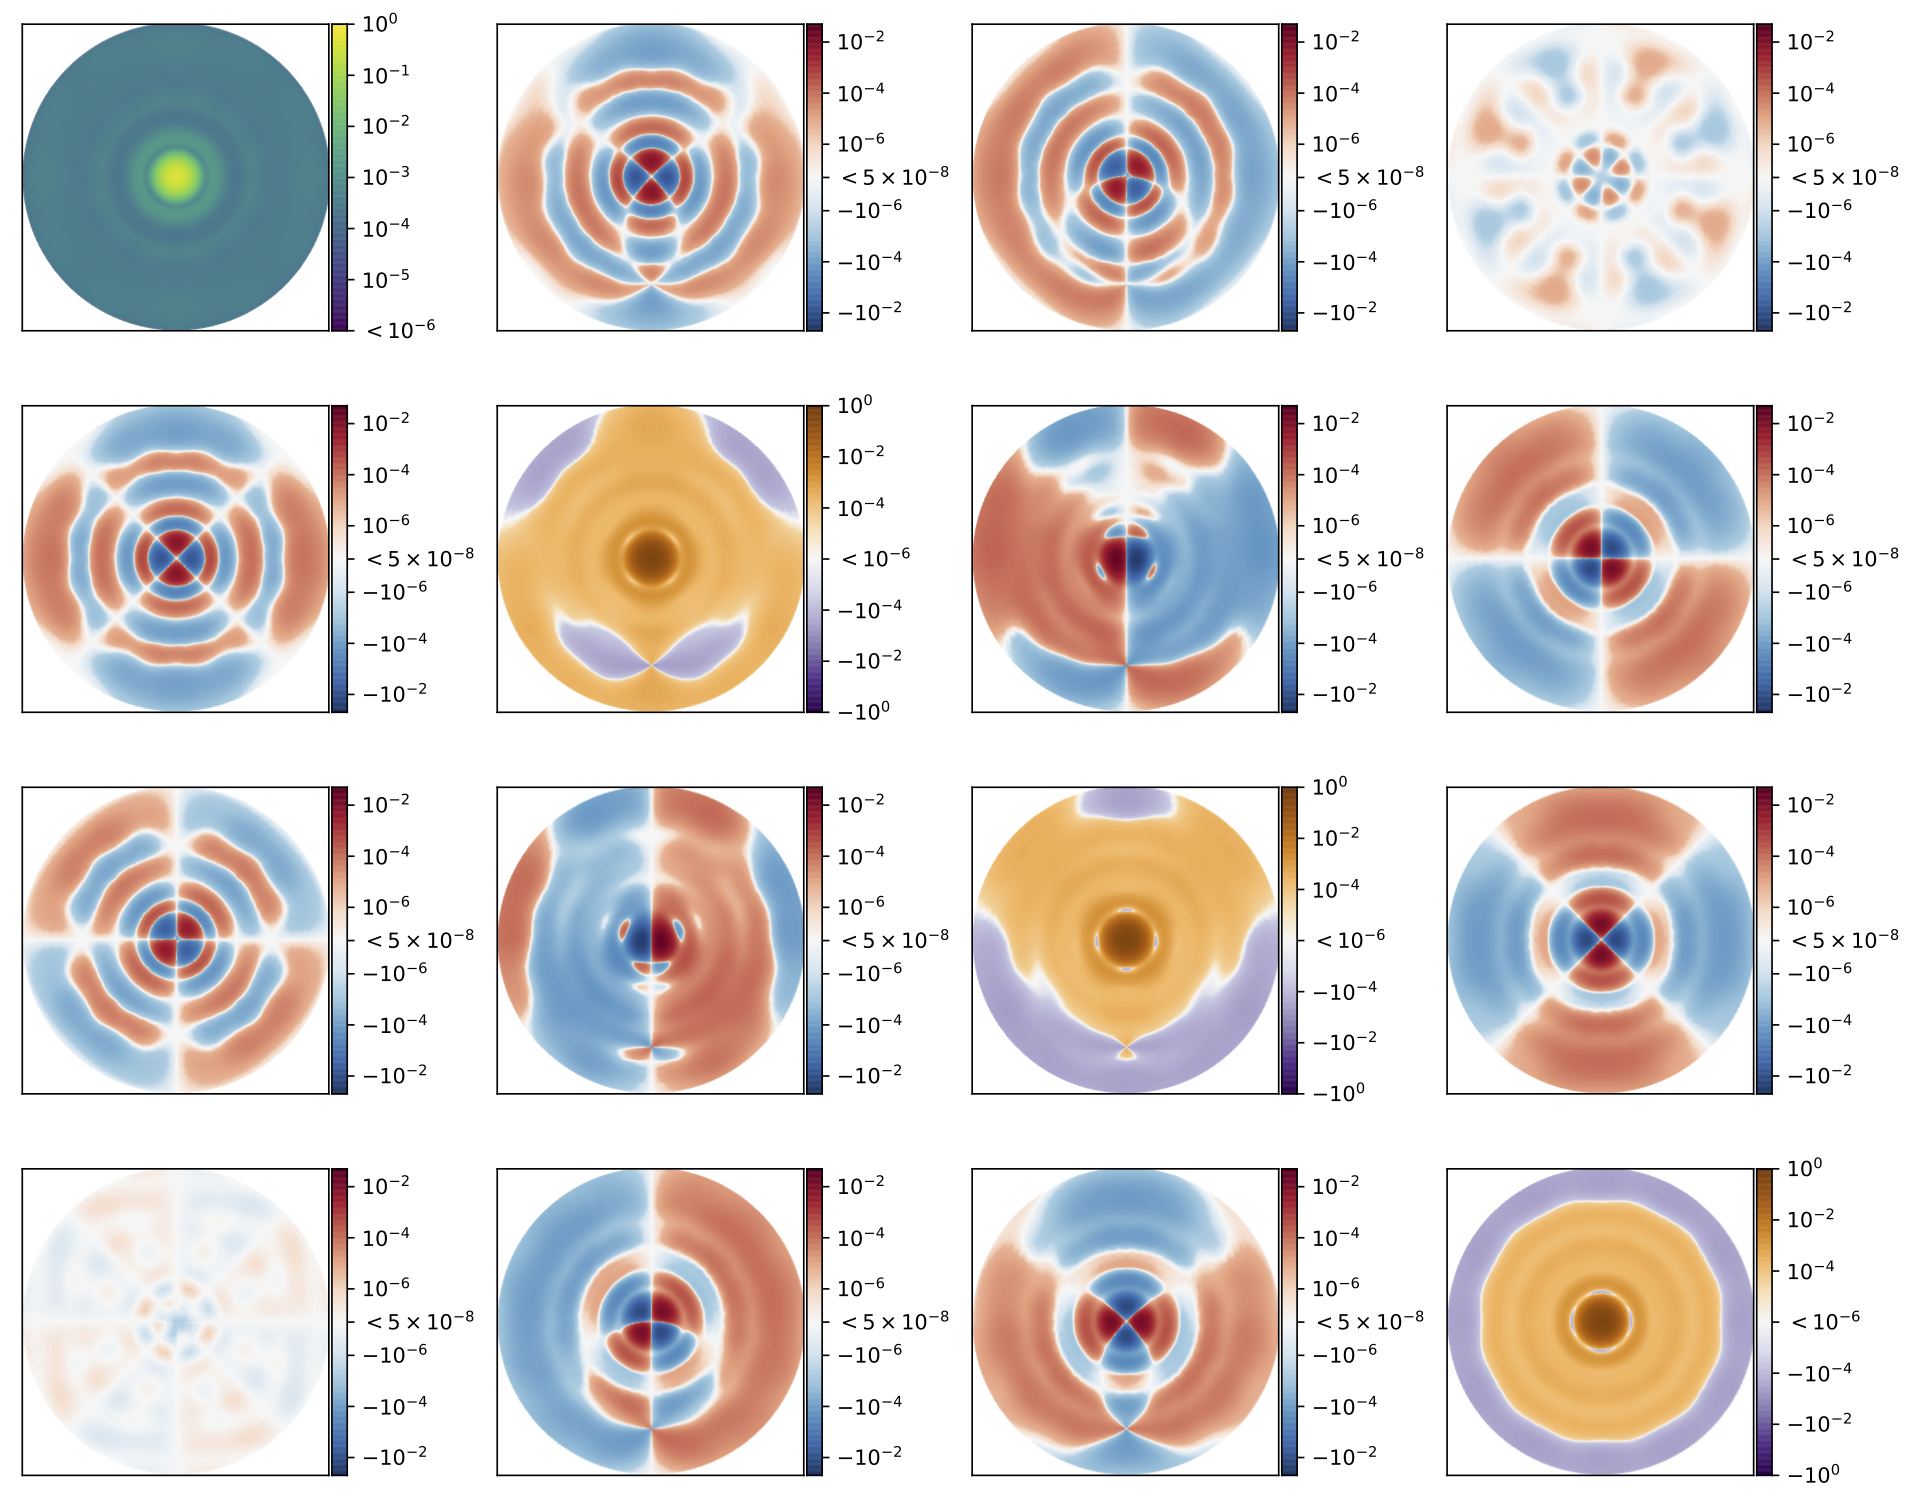
\includegraphics[scale=0.4]{full_mueller_120MHz.png}
\par\noindent\rule{0.8\textwidth}{0.4pt}
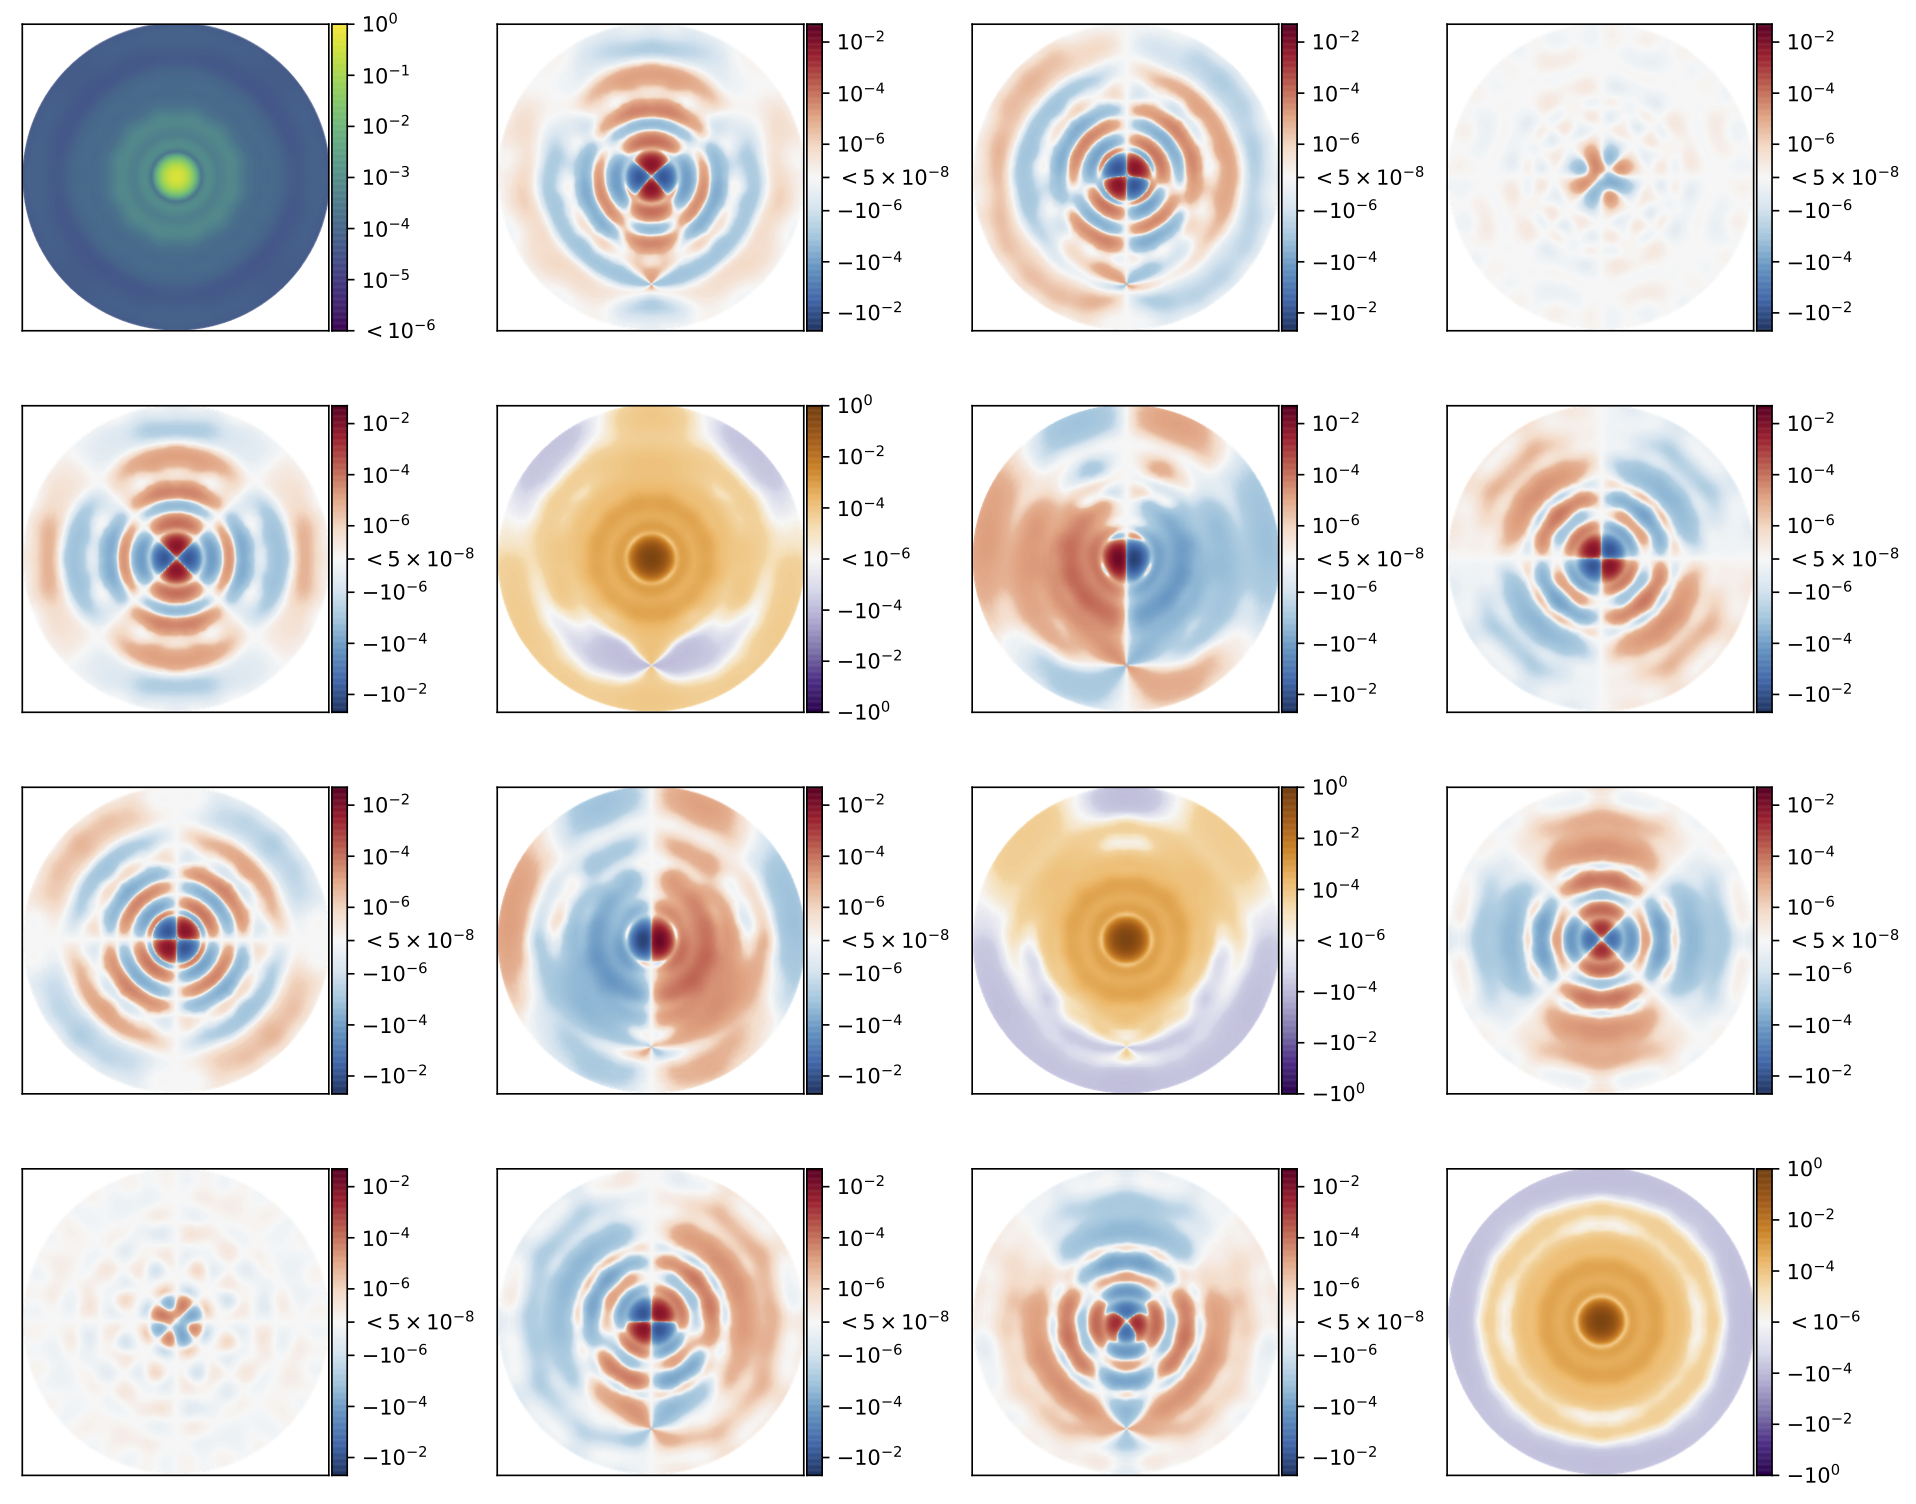
\includegraphics[scale=0.4]{full_mueller_160MHz.png}
\caption{Simulations of the instrumental direction dependent Mueller matrix at 120 MHz and 160 MHz (\textit{above} and \textit{below}, respectively) projected into the RA, Dec basis. Color scales for frequencies are relative to the peak of $\mathcal{M}_{00}$ (which itself is normalized to 1 at zenith). To account for the wide variety of dynamic ranges required to show detail, we use separate color maps for $\mathcal{M}_{00}$, diagonal, and off-diagonal terms. The off-diagonal terms are 2- to 8-orders of magnitude less than the diagonal terms. For a key to these matrices, see Equation~\ref{eq:Mab}.
}
\label{fig:mueller}
\end{figure*}

\begin{figure}
\centering
\hspace{-0.5cm}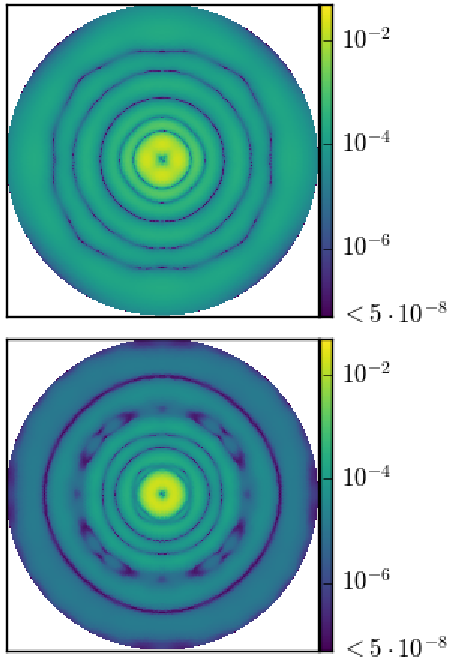
\includegraphics[scale=0.6]{M_p.pdf}
\caption{\edited{The magnitude of the linear polarization leakage beam given by $\mathcal{M}_p = \sqrt{\mathcal{M}_{IQ}^2 + \mathcal{M}_{IU}^2}$, or the middle two entries of the top row of Figure \ref{fig:mueller}, at 120 MHz and 160 MHz (\textit{above} and \textit{below}, respectively).
%A different view of the direction dependent Mueller matrix at 120 MHz and 160 MHz (\textit{above} and \textit{below}, respectively).   The left column is $\mathcal{M}_{II}$ (upper left corner of Figure \ref{fig:mueller}); the right column plots the spin-2 function $\mathcal{M}_{IQ} + i \mathcal{M}_{IU}$ with a color scale for the magnitude and a marker for the orientation.
%has a color scale given by $\mathcal{M}_p = \sqrt{\mathcal{M}_{IQ}^2 + \mathcal{M}_{IU}^2}$ and the marker indicates the orientation of the spin-2 function $M_{IQ} + i M_{IU}$.
}}
\label{fig:lin_pol_beam}
\end{figure}


At low frequencies and the large scales probed by many low frequency interferometers, Stokes I is extremely bright compared to the other Stokes parameters \citep{Bernardi.09, Bernardi.10, Jelic.14, Jelic.15, Asad15, Kohn16, Lenc.17, Moore17}. Moreover, only a few polarized point sources have been observed at frequencies below 300 MHz \citep{Bernardi.13, Asad.16, Lenc.17}. \cite{Farnes.14} showed evidence for systematic depolarization of steep-spectrum point sources towards low frequencies, causing low polarization fractions ($\ll 1\%$) below 300 MHz. 

\edited{The ``linear polarization leakage beam'' is shown for the two central frequencies of this analysis in Figure \ref{fig:lin_pol_beam}.   This quantity is the magnitude of the spin-2 function $\mathcal{M}_{IQ} + i \mathcal{M}_{IU}$ and represents the amplitude of the direction-dependent leakage of Stokes Q and U into I.}

These factors make the \edited{first row of $\mathcal{M}$, which represents $I\rightarrow V^I,\,V^Q,\,V^U,\,V^V$,} the most interesting for low-frequency polarized power spectra, since with limited calibration we can expect leakage from Stokes I into the other Stokes parameters to dominate over Stokes Q, U, and V emission alone. 

\edited{We produced simulations $\mathcal{V}$ using our fully-polarized formalism for the HERA-19 commissioning array, described below, using an unpolarized model of the low frequency sky from the Global Sky Model \citep[GSM;][]{GSM.08, pygsm, GSM.17} at the appropriate R.A. range to match our observations. These simulations are based on the same source code }

Forming power spectra from these visibilities allowed for a comparison of our data to a ``leakage only'' regime. We discuss the process for forming power spectra in Section~\ref{subsec:pspec}, and the simulated power spectra are shown in comparison to those from data in Section~\ref{sec:results}.

\subsection{Direction-Independent Leakage}
\label{subsec:DI-Leak}

% I think you are using "ideal dipoles" to mean "ideal polarization feeds", but the ideal dipole does NOT have ideal polarization response.
%If ideal dipoles were achievable, one could completely isolate Stokes parameters in the pseudo-Stokes visibilities \citep{Hamaker.96, TMS, Moore13}:
In addition to the mixing of Stokes parameters due to the primary beam, it is possible to mix them in a direction independent way. Calibration errors are capable of leaking signal between pseudo-Stokes visibilities independent of the sky \citep{TMS}. Again focusing on the $\{V^I,\,V^Q,\,V^U,\,V^V\}$ components of this leakage, we have:
\begin{itemize}
\item $V^I \rightarrow V^Q$ occurs through errors in calibrating the complex voltage gain factors for each dipole arm.
\item $V^I \rightarrow V^U$ occurs through the sum of off-diagonal gain terms (\textit{D}-terms; the receptivity of dipole arm ``n'' to an electric field vector aligned with arm ``e'' and vice versa).
\item $V^I \rightarrow V^V$ occurs through the difference in \textit{D}-terms between two feeds.
\end{itemize}

% We need to make clear that the simulations don't "need" diagonal gain errors, because nominally we correct for them.  
We neglect calibration errors, and hence direction-independent leakage, in our simulations in order to build intuition around power spectrum estimates for a ``perfectly behaving'' instrument.  

\section{Observations and Reduction}
\label{sec:obs}

In this work we used eight nights of observations from the HERA-19 commissioning array. HERA is a low-frequency interferometer composed of 14\,m-diameter dishes arranged in a close-packed hexagonal array of 14.7\,m spacing. The commissioning array consists of nineteen dishes (see Figure~\ref{fig:antpos}); HERA is being constructed in staged build-outs, and upon completion will consist of 350 dishes in a fractured hexagon configuration \citep[see][]{DillonParsons16, deBoer17}. A feed cage containing two dipole feeds (recycled from the PAPER array, see \citealt{Parsons.10}), oriented in North-South and East-West directions, was suspended above each dish \citep{Neben.16,Ewall-Wice.16,Thyagarajan.16}.

HERA only observes in drift-scan mode. The observations we used were eight nights, from Julian Date (JD) 2457548 to 2457555; LSTs 10.5 -- 23 hr. Drift-scan visibilities were recorded every 10.7 seconds for 1024 evenly-spaced channels across the 100-200\,MHz bandwidth. These data were divided into {\sc miriad} data sets roughly 10 minutes long. A night's observation lasted 12 hours in total (6pm to 6am South African Standard Time; SAST); of these we used the central 10 hours, to avoid the sun. \edited{The details of our observations are summarized in Table~\ref{tab:params}.}

\begin{figure}
\centering
\hspace{-0.5cm}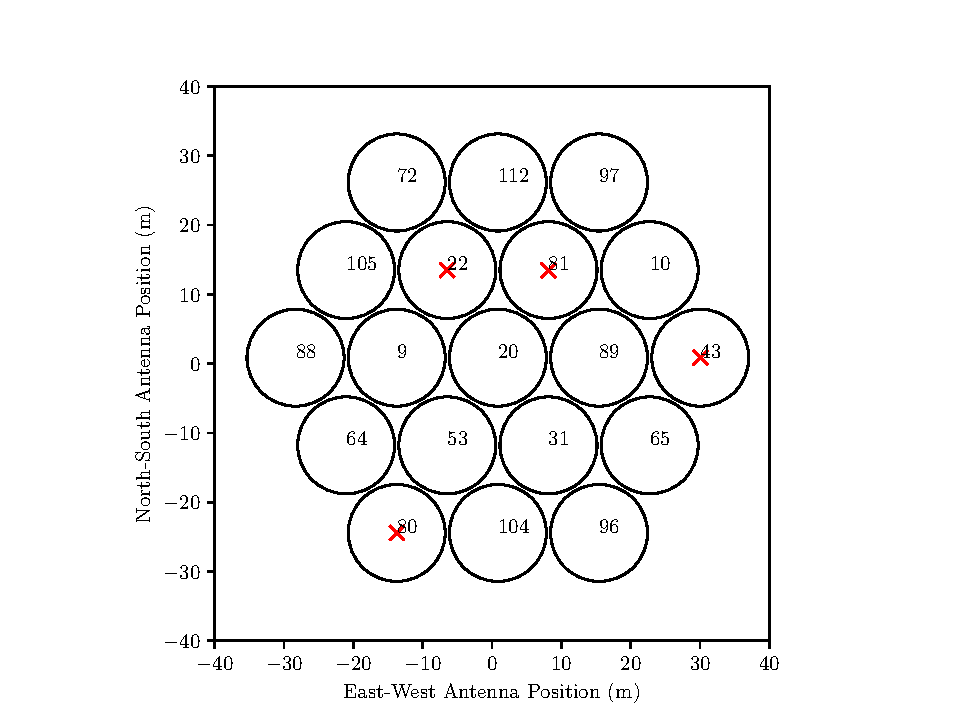
\includegraphics[scale=0.6]{antpos_hera19.pdf}
\caption{\edited{The configuration of the HERA-19 array.} The perimeter of each dish \edited{is shown as a circle.} 
A red ``X'' marks antennae that were identified during preprocessing and calibration as malfunctioning and were excluded from further analysis.}
\label{fig:antpos}
\end{figure}


\begin{table}
\centering
\caption{\edited{Observational parameters used for this study.}}
\begin{tabular}{lc}
\hline
Parameter & Value \\
\hline
Array location & 30:43:17.5$^\circ$ S, 21:25:41.9$^\circ$ E \\
JD range & 2457548 -- 2457555 \\
LST Range & 10.6 -- 23 hrs \\
Frequency range & 115 -- 185 MHz \\
Frequency resolution & 97.6 kHz \\
Integration time & 10.7 s\\
Element diameter & 14.0 m\\
Number of elements & 15 \\
Shortest baseline & 14.6 m \\
Longest baseline & 58.4 m \\
%Multi-frequency synthesis beam diameter & 2\arcdeg \\
Primary beam diameter & $9^{\circ}$ \\
System Temperature & $100 + 120(\nu / 150\,{\rm MHz})^{-2.55}$ K\\
SEFD per element & $\sim 5800$ Jy at 150 MHz\\

\hline
\end{tabular}
\label{tab:params}
\end{table}

\edited{\subsection{RFI Excision and Flagging}}

To identify samples contaminated by radio frequency interference (RFI), a two-dimensional median filter in time and frequency was applied to the visibility data to smooth out high pixel-to-pixel variations, and remove significant outliers that were likely unphysical. The variance of the resulting data was computed, and points with a $z$-score greater than 6 (i.e., points where the value is more than 6$\sigma$ away from the mean) were flagged as initial seeds for RFI extraction. A two-dimensional watershed algorithm was applied using these seeds as starting points, enlarging the regions of RFI-contamination to neighboring pixels with $z$-scores greater than 2, until all such pixels were flagged. Figure~\ref{fig:rfi} shows the fractional RFI flag occupancy per time (displayed in LST) and frequency across the 8 days of observations. The majority of the band is relatively clear of RFI. Some clear features are: the FM radio band (below 110 MHz), ORBCOMM satellite communications (137 MHz), an ISS downlink (150 MHz) and VHF TV channels (above 170 MHz)\footnote{For an extended discussion of RFI as seen by HERA, see the public \href{http://reionization.org/wp-content/uploads/2013/03/HERAMemo19_HERA_dish_RFI.pdf}{\edited{\underline{HERA Memo \#19}}}}.
The galaxy, when transiting zenith at LST$\approx$17.75 hours, is so bright that it appears to degrade our ability to flag RFI.

\edited{Four antennae were identified during the commissioning as having anomalous behavior. These are marked with red ``X''s in Figure~\ref{fig:antpos} and were omitted from further analysis.  Before calibration, we manually flagged the edges of the band (below 110 MHz and above 190 MHz), where spectral behavior is dominated by the high and low pass filtering in the HERA signal chain \citep{deBoer17}.}

\begin{figure}
\centering
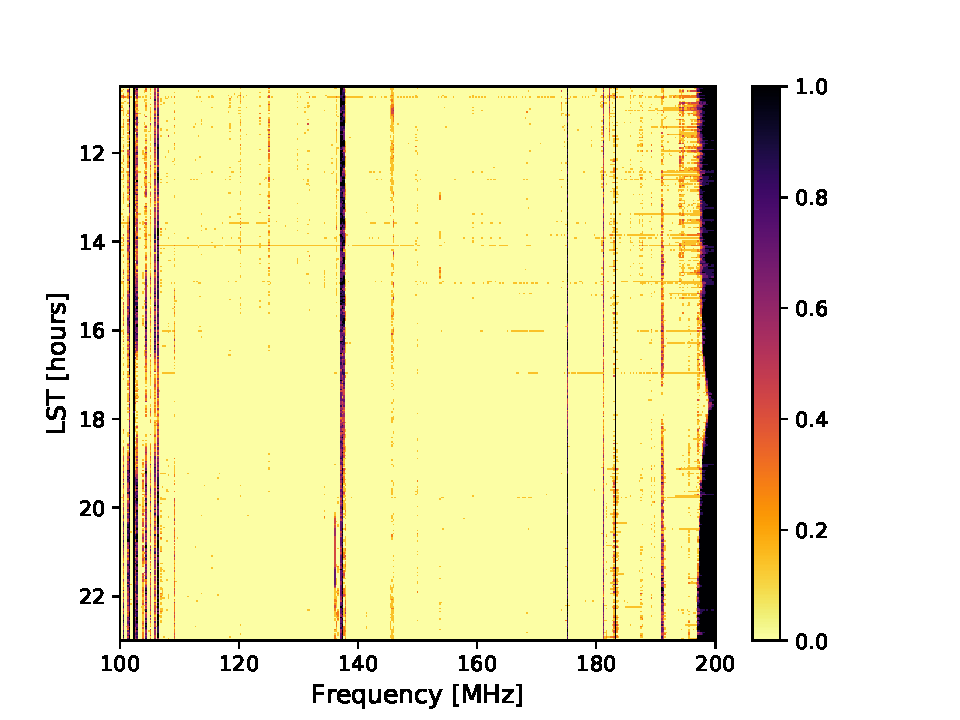
\includegraphics[scale=0.6]{frac_occ.pdf}
\caption{Fractional RFI flag occupancy per time and frequency over the eight days of observations. RFI was flagged on a per-(time,frequency) sample basis.}
\label{fig:rfi}
\end{figure}

\subsection{Calibration}
\label{subsec:cal}

HERA is designed to be calibrated using redundant calibration techniques \citep{DillonParsons16}, but for this preliminary view of HERA commissioning data, we used image-based calibration. Future studies with deeper integrations targeting EoR detections will take advantage of redundancy to obtain more precise calibration solutions \citep{deBoer17}. We used the \casa\ \citep{casa} package for calibration, taking advantage of its CLEAN, {\tt gaincal} and {\tt bandpass} functions.  \edited{We first converted from HERA's native {\sc miriad} to a {\sc uvfits} file format using {\sc pyuvdata} \citep{pyuvdata}; this could then be ingested by \casa.}

\edited{The brightest calibration sources near the Dec -30\arcdeg\ stripe -- for example, those used in previous PAPER analyses like Pictor A \citep{jacobs13b} -- were not available for this observing window (10.5 - 23 h RA), and the few long baselines in the array available made calibration using individual fainter point sources difficult.  We therefore developed a calibration method using the Galactic Center (GC; taken to be at $\alpha, \delta$ = 17h 45m 40s, -29d 0m 28s) as modeled by the GSM. Specifically, we selected four minutes of data centered at the transit of the GC to use for calibration.   The visibilities were phased from drift-scan mode to a single phase center chosen to be the LST at the start of the observations.  Because this phasing imperfectly approximates the tracking telescope assumed by \casa, the length of the observation was chosen to minimize the effects of beam-dependent gain variations as the GC transited.  The calibration was done as a two-step process.  First, we built an initial model with the GC as an unpolarized, flat-spectrum source with flux density scaled to a reference point of 1 Jy.  This allowed us to solve for the large antenna based delay terms using {\tt gaincal} ({\tt gaintype='K'}; typically 10's of ns) and a complex bandpass using {\tt bandpass}.  A single solution was obtained for the 4 minute observation for both calibration types, and for the bandpass a solution was obtained for each unflagged $\sim$100 kHz channel, resulting in a complex, frequency-dependent gain for each feed.	With this first calibration in place, the second step was to interactively CLEAN the image to obtain a more accurate model of the GC extended structure.  We still assumed an unpolarized source, but allowed multiple components within a two degree radius centered on the GC.  This was followed by a second round of delay and bandpass calibration to the multi-component extended model, completely analogous to first round of calibration.  At this point, an overall frequency-dependent amplitude was required to scale the gains from the arbitrary 1 Jy normalization.  For this we used our simulation of the GC from the GSM (converted to units of Jy) to determine a single, spectrally-smooth function for all antennas to make the spectrum of the observations match the simulations.

Clearly, this is an incomplete calibration model. The assumption that the GC is unpolarized is probably adequate, due to the large optical depth towards the GC \citep{Oppermann.12} resulting in near-complete depolarization in the plane of the Galaxy \citep{Wolleben.06}.  Moreover, we expect significant beam depolarization due to the large solid angle of the synthesized beam (see Table \ref{tab:params}).
%(about 2\arcdeg\ FWHM).  
Other assumptions are less obviously correct: 
the GC structure is only partially modeled, and we have assumed the GSM provides an accurate calibration.  We have also assumed that the direction-independent Jones matrix is diagonal; we did not attempt to obtain \textit{D}-terms.  However, as the objective of this work is to explore the response of the instrument in power spectrum space without combining baselines of different lengths, most of the purpose of the calibration is to correct an initial large cable delay per antenna to align all of the power spectra at zero delay, and to set the overall flux scale.  The limited our interpretive power for addressing some aspects of polarization leakage, which we discuss in Section~\ref{sec:results}.

The resulting gains are shown in Figure~\ref{fig:bandpass}.  The gain amplitudes are clearly very similar in shape, with one outlier, and they cluster with 25\% of each other.  After removing the phase due to the delay term, the resulting phases show only small variations around their mean.  The derived bandpasses are clearly spectrally smooth, and thus, even if there are errors, we expect that they will not add additional spectral structure to the power spectrum (see Section \ref{subsec:pspec}).  These gains were applied to all 8 nights of observations. It was found that this produced smaller day-to-day calibration variability than calibrating each day separately to the GC; see Section \ref{subsec:variability}.   


\begin{figure}
\centering
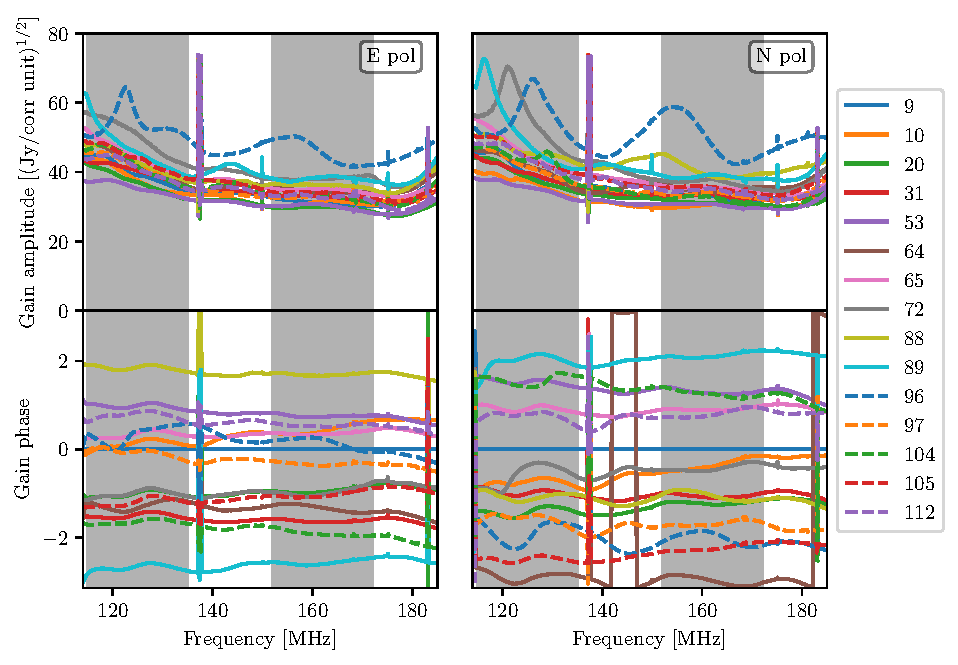
\includegraphics[scale=0.5]{gains.pdf}
%{h19_2457458_abs_smallzoom_nolegend.png}
\caption{\edited{Bandpass solutions obtained for both dipole orientations for all functioning antennae in the array on JD 2457548, and subsequently applied to all data.  Each antenna is marked by a different line color and style. Shaded regions indicate the effective sub-bands (the 10 MHz at the center of the 20 MHz Blackman-Harris window) used for power spectrum analysis.  The phase is shown after the removal the delay term.}}
\label{fig:bandpass}
\end{figure}


Figure~\ref{fig:phasecal} shows the effect of calibration on the visibilities of three nominally redundantly-spaced baselines.  Shown in that figure are the phases of three $V^{nn}$ visibilities from 14.7\,m baselines before and after calibration. There were no shared antennae between the visibilities shown. The qualitative agreement is obvious, providing a consistency check on the solutions, and showing our sky-based model is achieves redundancy without assuming it.  However, small-scale variations between baselines are still seen.  This not unexpected; the antennas are likely to be non-identical, and we have evidence based on closure phase (which is insensitive to calibration errors) that redundant baselines do not see the sky identically \citep{carilli18}.   

\begin{figure}
\centering
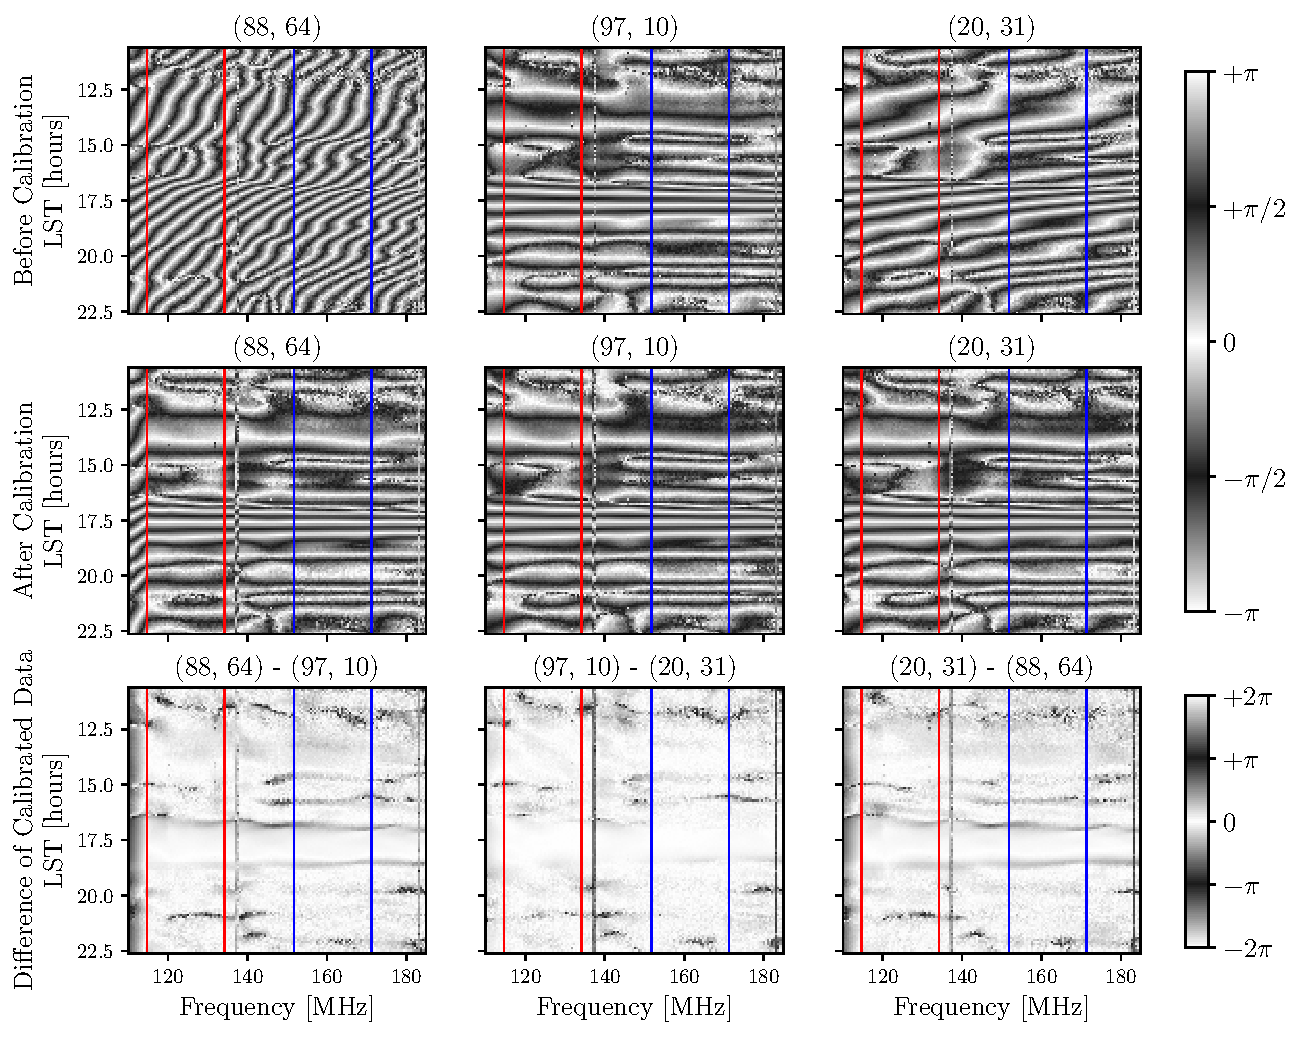
\includegraphics[scale=0.38]{calibration_on_phases_noflags.pdf}
\caption{
The effect of calibration on the phases of visibilities from three redundantly-spaced 14.7\,m baselines; \textit{nn} polarization. 
The antenna numbers refer to those given in Figure \ref{fig:antpos}.
The color scale is cyclic; black is $\pm\pi/2$ and white is 0 and $\pm\pi$. The extend of the low band is indicated with red lines and the high band with blue.  
\textit{Top row}: before calibration; \textit{Middle row}: after calibration; \textit{Bottom row}: the three pairs of differences of the calibrated phases.  
Note that the agreement between baselines is excellent near the Galactic Center but shows significant differences at some other times.
}
\label{fig:phasecal}
\end{figure}

In Figure~\ref{fig:GCimage}, we show images formed from the simulated pseudo-Stokes visibilities (top panels) and our observations (bottom panels). 
These are multi-frequency synthesis images, where we used all unflagged frequencies on either side of the band edges, from 115 MHz to 188 MHz.  
The primary beam has not been deconvolved. 
All images shown were produced using the same four minute interval used for calibration.
Note that at HERA's latitude the Galactic Center transits 2\arcdeg\ north of zenith, while the HERA primary beam has a FWHM of $\sim5\arcdeg$ at 150\,MHz \citep{Neben.16}. For the simulated visibilities, we flagged the same antennae and channels as in the data. As expected for a compact array, the Stokes I images capture only a low-resolution view of the Galactic Center. The simulated and observed visibilities form remarkably similar images in Stokes I, and Q and U clearly share features in common, due to leakage from I to Q and U through the primary beam (recall that the simulations are unpolarized).  In Stokes V,  the simulation notably does not reproduce the image well. 
The presence of emission at the location of the Galactic Center not due to primary beam leakage is consistent with direction-independent gain errors at the few percent level in amplitude (for Stokes Q) and D-terms at $\sim 1\%$ relative to the diagonal gains (for Stokes V) \citep{TMS}.  Note that the Stokes U image is broadly consistent with a large fraction of power coming from I leakage through the primary beam, though there is some additional power as well.  We consider the implications for the power spectrum in Section~\ref{sec:results}.
}

\begin{figure*}
\centering
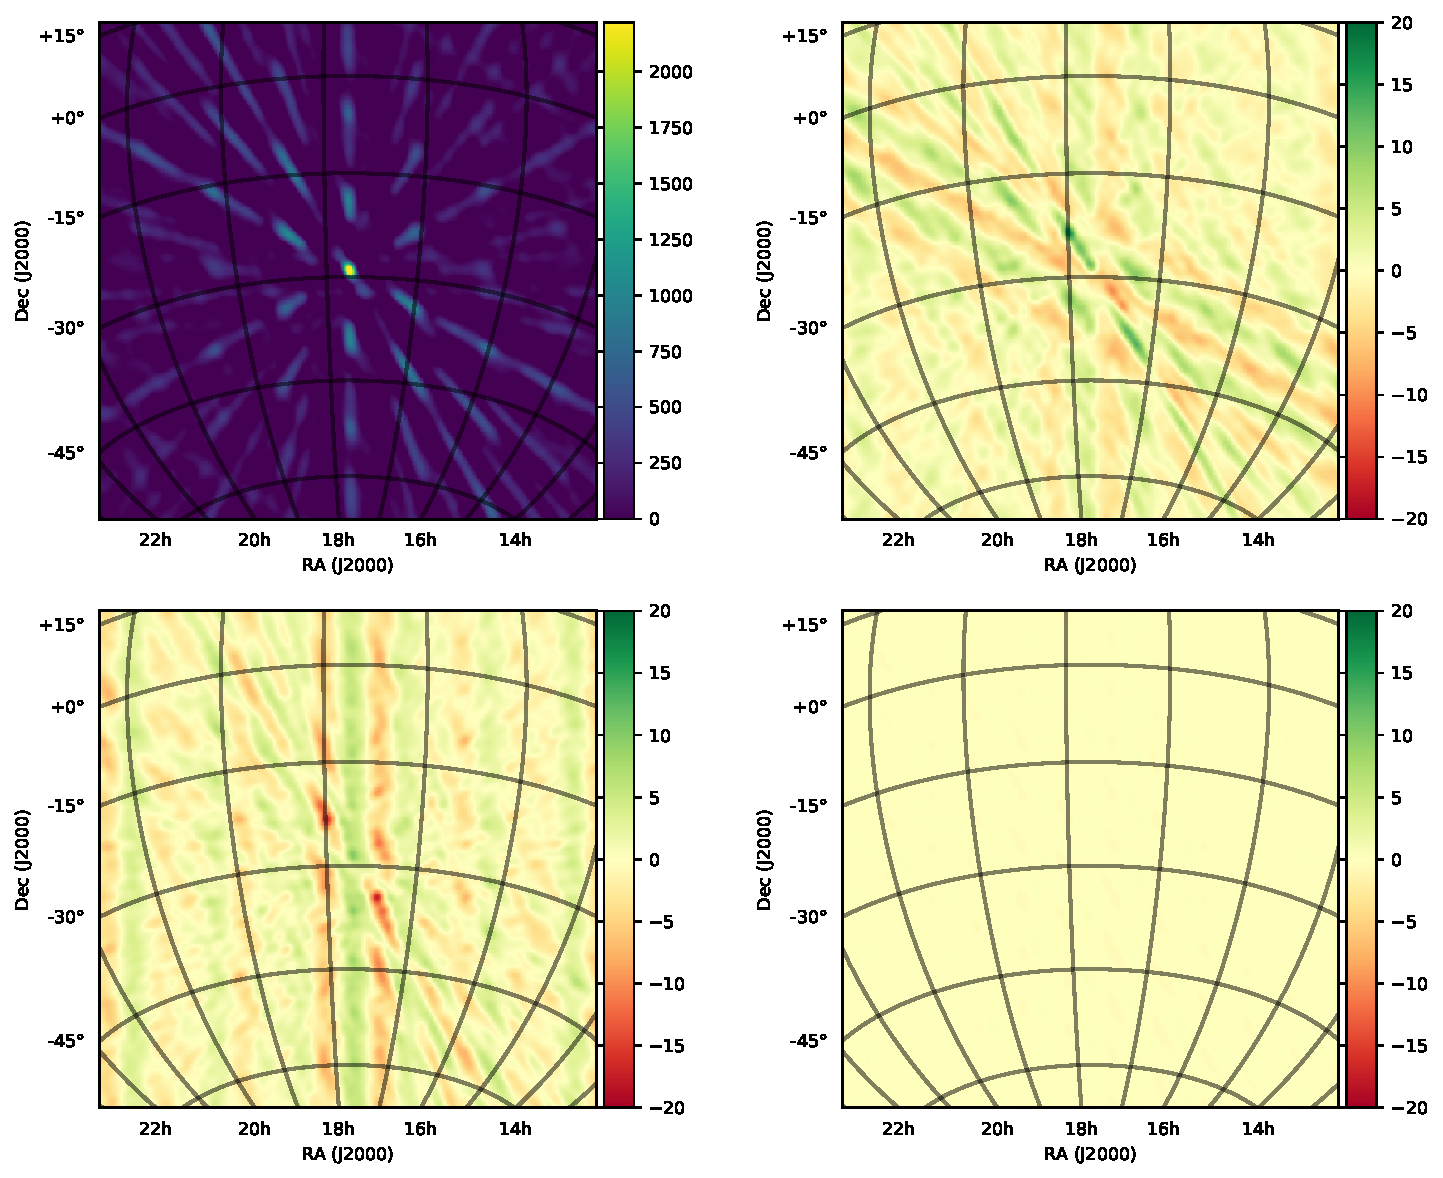
\includegraphics[width=0.7\textwidth]{sim4pol_new.pdf}
%{sim4pol.pdf}
\vspace{-0.1in}
\par\noindent\rule{0.8\textwidth}{0.4pt}
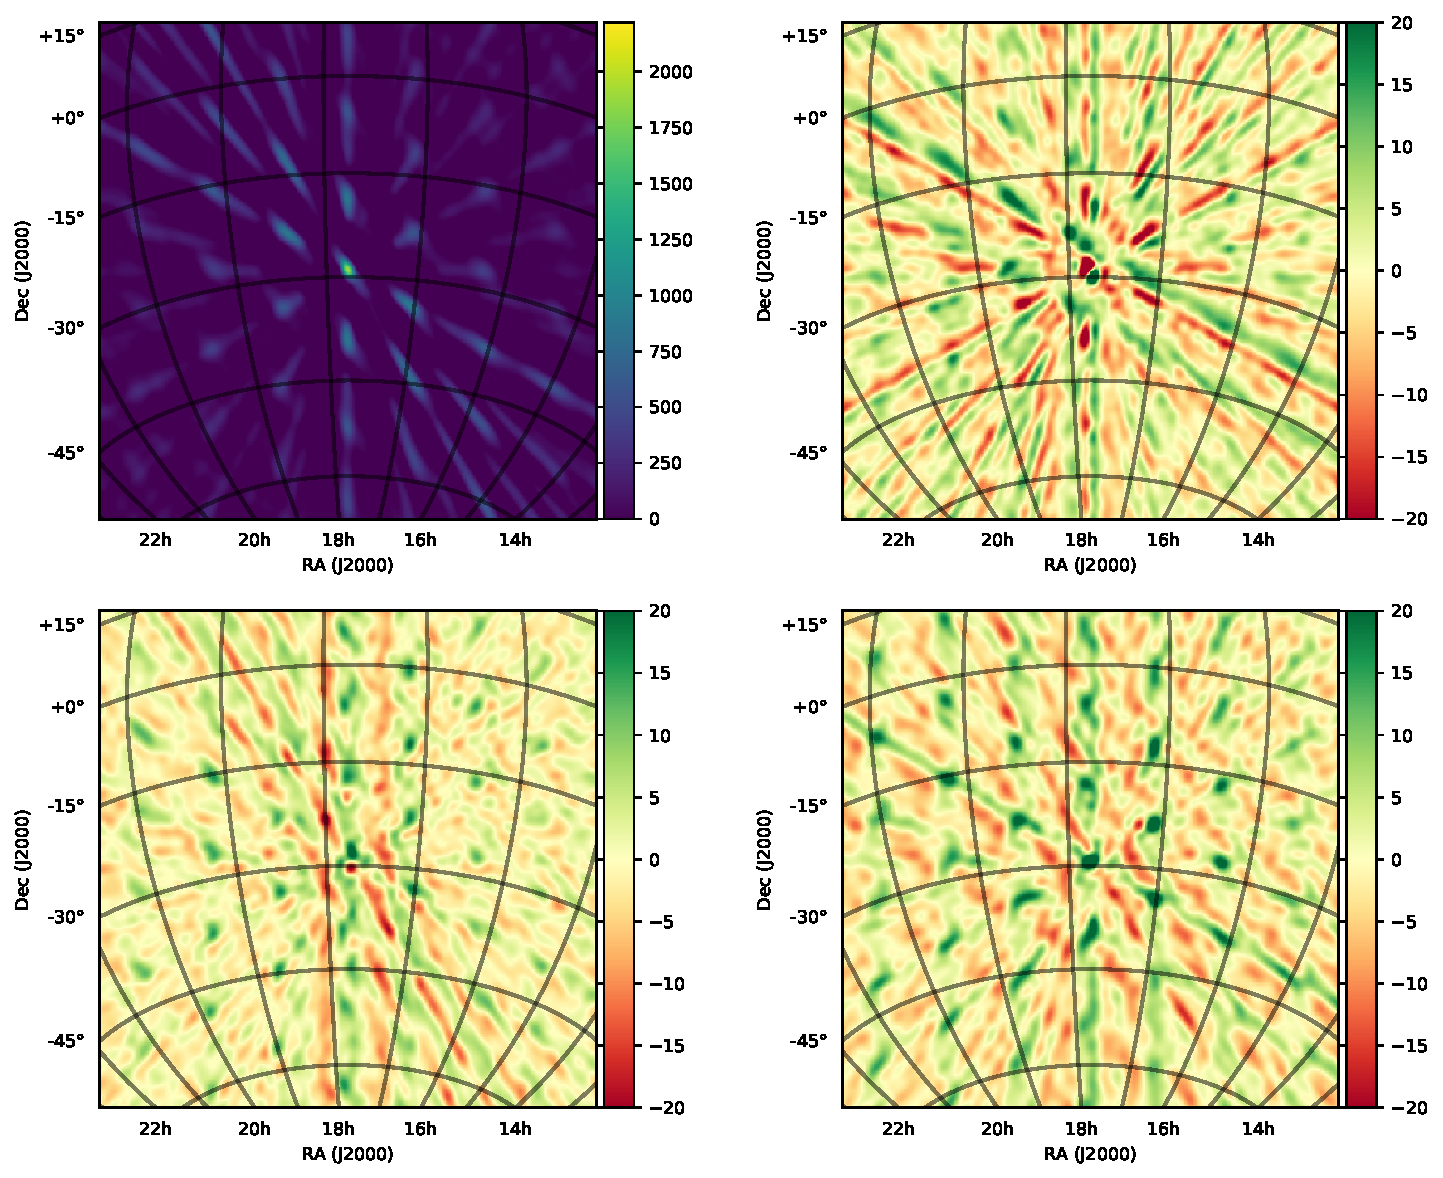
\includegraphics[width=0.7\textwidth]
{real4pol_new.pdf}
%{new4pol.pdf}
\caption{\edited{
Both sets of panels show multi-frequency synthesis pseudo-Stokes images of I, Q, U and V visibilities (\textit{top left, top right, lower left, lower right}) for the Galactic Center (our calibration source) at transit.  Note the field-of-view show is about 60\arcdeg across.
A Briggs-weighting with robustness 0 was used when gridding into the image plane. 
No deconvolution was performed. 
The colorbar is in units of Jy/Beam.
A separate color scale is used for Stokes I for suitable dynamic range in the polarized fluxes; note that the color scales differ by a factor of 100.
\textit{Above}:  Simulation, where only a Stokes I sky was used; any polarized power is due to direction-dependent polarization leakage (see Section~\ref{subsec:DD-Leak}).
\textit{Below}: Multi-frequency synthesis pseudo-Stokes images formed from observed visibilities on JD 2457548.
}
}
\label{fig:GCimage}
\end{figure*}


\subsection{Forming power spectra}
\label{subsec:pspec}

Power spectra were formed according to the method used in \cite{Pober13} and \cite{Kohn16}, which we briefly review here. \cite{Parsons.12a} define the \textit{delay transform} as the Fourier transform of a visibility for baseline $ij$ and pseudo-Stokes parameter $P$ along the frequency axis
\begin{equation}
\label{eq:DelaySpectrum}
\tilde{V}_{ij}^{P}(\tau, t) = \int {\rm d}\nu \tilde{V}_{ij}^{P}(\nu, t)e^{2\pi i \nu \tau}.
\end{equation}

\edited{
We selected two relatively RFI-free 20 MHz sub-bands (Figure~\ref{fig:rfi}); 115 to 135 MHz and 152 to 172 MHz, henceforth referred to the ``low band'' and the ``high band'' in which to compute the power spectrum. The bands were multiplied by a Blackman-Harris window, centered on their central frequencies, before Fourier transforming, in order to minimize side-lobes. This windowing led to an noise-effective bandwidth of 10 MHz.  We note that this bandwidth is appropriate for EoR analyses since the {\sc Hi} signal is, to a reasonable approximation, coeval over the corresponding redshift range \citep{Furlanetto06}.  However, this resolution (approximately 100 ns in delay as compared to 194 ns for the longest baseline in this study) does limit our ability to resolve certain features in the power spectrum. 
We also note that using a Blackman-Harris window will induce a correlation between adjacent $\tau$ modes; this should be borne in mind when interpreting plots, as all delay bins are plotted.}

The power at each delay-mode and baseline can be represented in terms of their respective Fourier components $k_{\parallel}$ and $k_{\perp}$ \citep{Parsons.12a, Nithya.15b}:
\begin{multline}
P(k_{\parallel},k_{\perp}) \approx | \tilde{V}_{ij}^{P}(\tau) |^2 \frac{X^2 Y}{\Omega B} \left(\frac{c^2}{2k_B\nu^2}\right)^2 , \\\\
k_{\parallel} = \frac{2\pi \nu_{\rm 21cm} H(z) %H_0 \sqrt{\Omega_m (1+z)^3 + \Omega_k (1+z)^2 + \Omega_{\Lambda}} 
}{c (1+z)^2}\tau, \\\\
k_{\perp} = \frac{2\pi}{D(z) \lambda} b\\
\end{multline}
for: bandwidth $B$, angular area of the beam $\Omega$, $\nu_{\rm 21cm}\approx$1420 MHz, baseline length $b$, wavelength of observation $\lambda$, Hubble parameter $H(z)$, transverse comoving distance $D(z)$ and redshift-dependent scalars X and Y \citep{Parsons.12b}. Note that the angular area of the beam refers to the diagonal components of the Mueller matrices shown in Figure~\ref{fig:mueller}. For further discussion of forming polarized power spectra in $k$-space, refer to \cite{Nunhokee.17}.

\edited{To avoid a noise bias when forming the power spectrum, 
we cross-multiplied consecutive integrations (each having independent noise)}, 
rephasing the zenith angle of the latter to the former:
\begin{equation}
\label{eq:adj_time_ps}
 | \tilde{V}_{ij}^{P}(\tau, t) |^2 \approx | \tilde{V}_{ij}^{P}(\tau, t) \times \tilde{V}_{ij}^{P}(\tau, t+\Delta t)e^{i\theta_{ij,\rm zen}(\Delta t)}|
\end{equation}
where $\theta_{ij,\rm zen}(\Delta t)$ was the appropriate phasing for baseline $ij$ and $\Delta t = 10.7$ seconds.

Pseudo-stokes power spectra were formed for each pair of integrations, for every baseline, \edited{according to Equation \ref{eq:adj_time_ps}.  Power spectra from baselines of identical lengths were then averaged together for all observation times}.  Appealing to cosmological isotropy, baselines of the same length but different orientation should be sampling the same cosmological structure.  
\edited{The resulting ``1D'' power spectra for each baseline length were then averaged over all eight days and concatenated to form a  two-dimensional power spectrum (that is, arranged into the ($k_{\perp}$, $k_{\parallel}$) plane).  Note that all averaging in this study was performed {\it after} forming power spectra, {\it not} by averaging visibilities; this incoherent averaging is non-optimal for achieving the greatest sensitivity in the EoR window.  However, the intention of this investigation was not a deep integration on noise, but rather a first look at calibration and foreground properties as observed through the polarized beam.}

\section{Results \& Discussion}
\label{sec:results}

\edited{The power spectra formed from the above procedure are shown f or all pseudo-Stokes parameters for the high and low bands in Figures~\ref{fig:pitchforks_highband} and \ref{fig:pitchforks_lowband}, respectively.   
%Note that the one- and two-dimensional presentations are the {\it same} data in middle and lower panels, with the presentation varied to make different features apparent.
} 

\begin{figure*}[h]
\centering
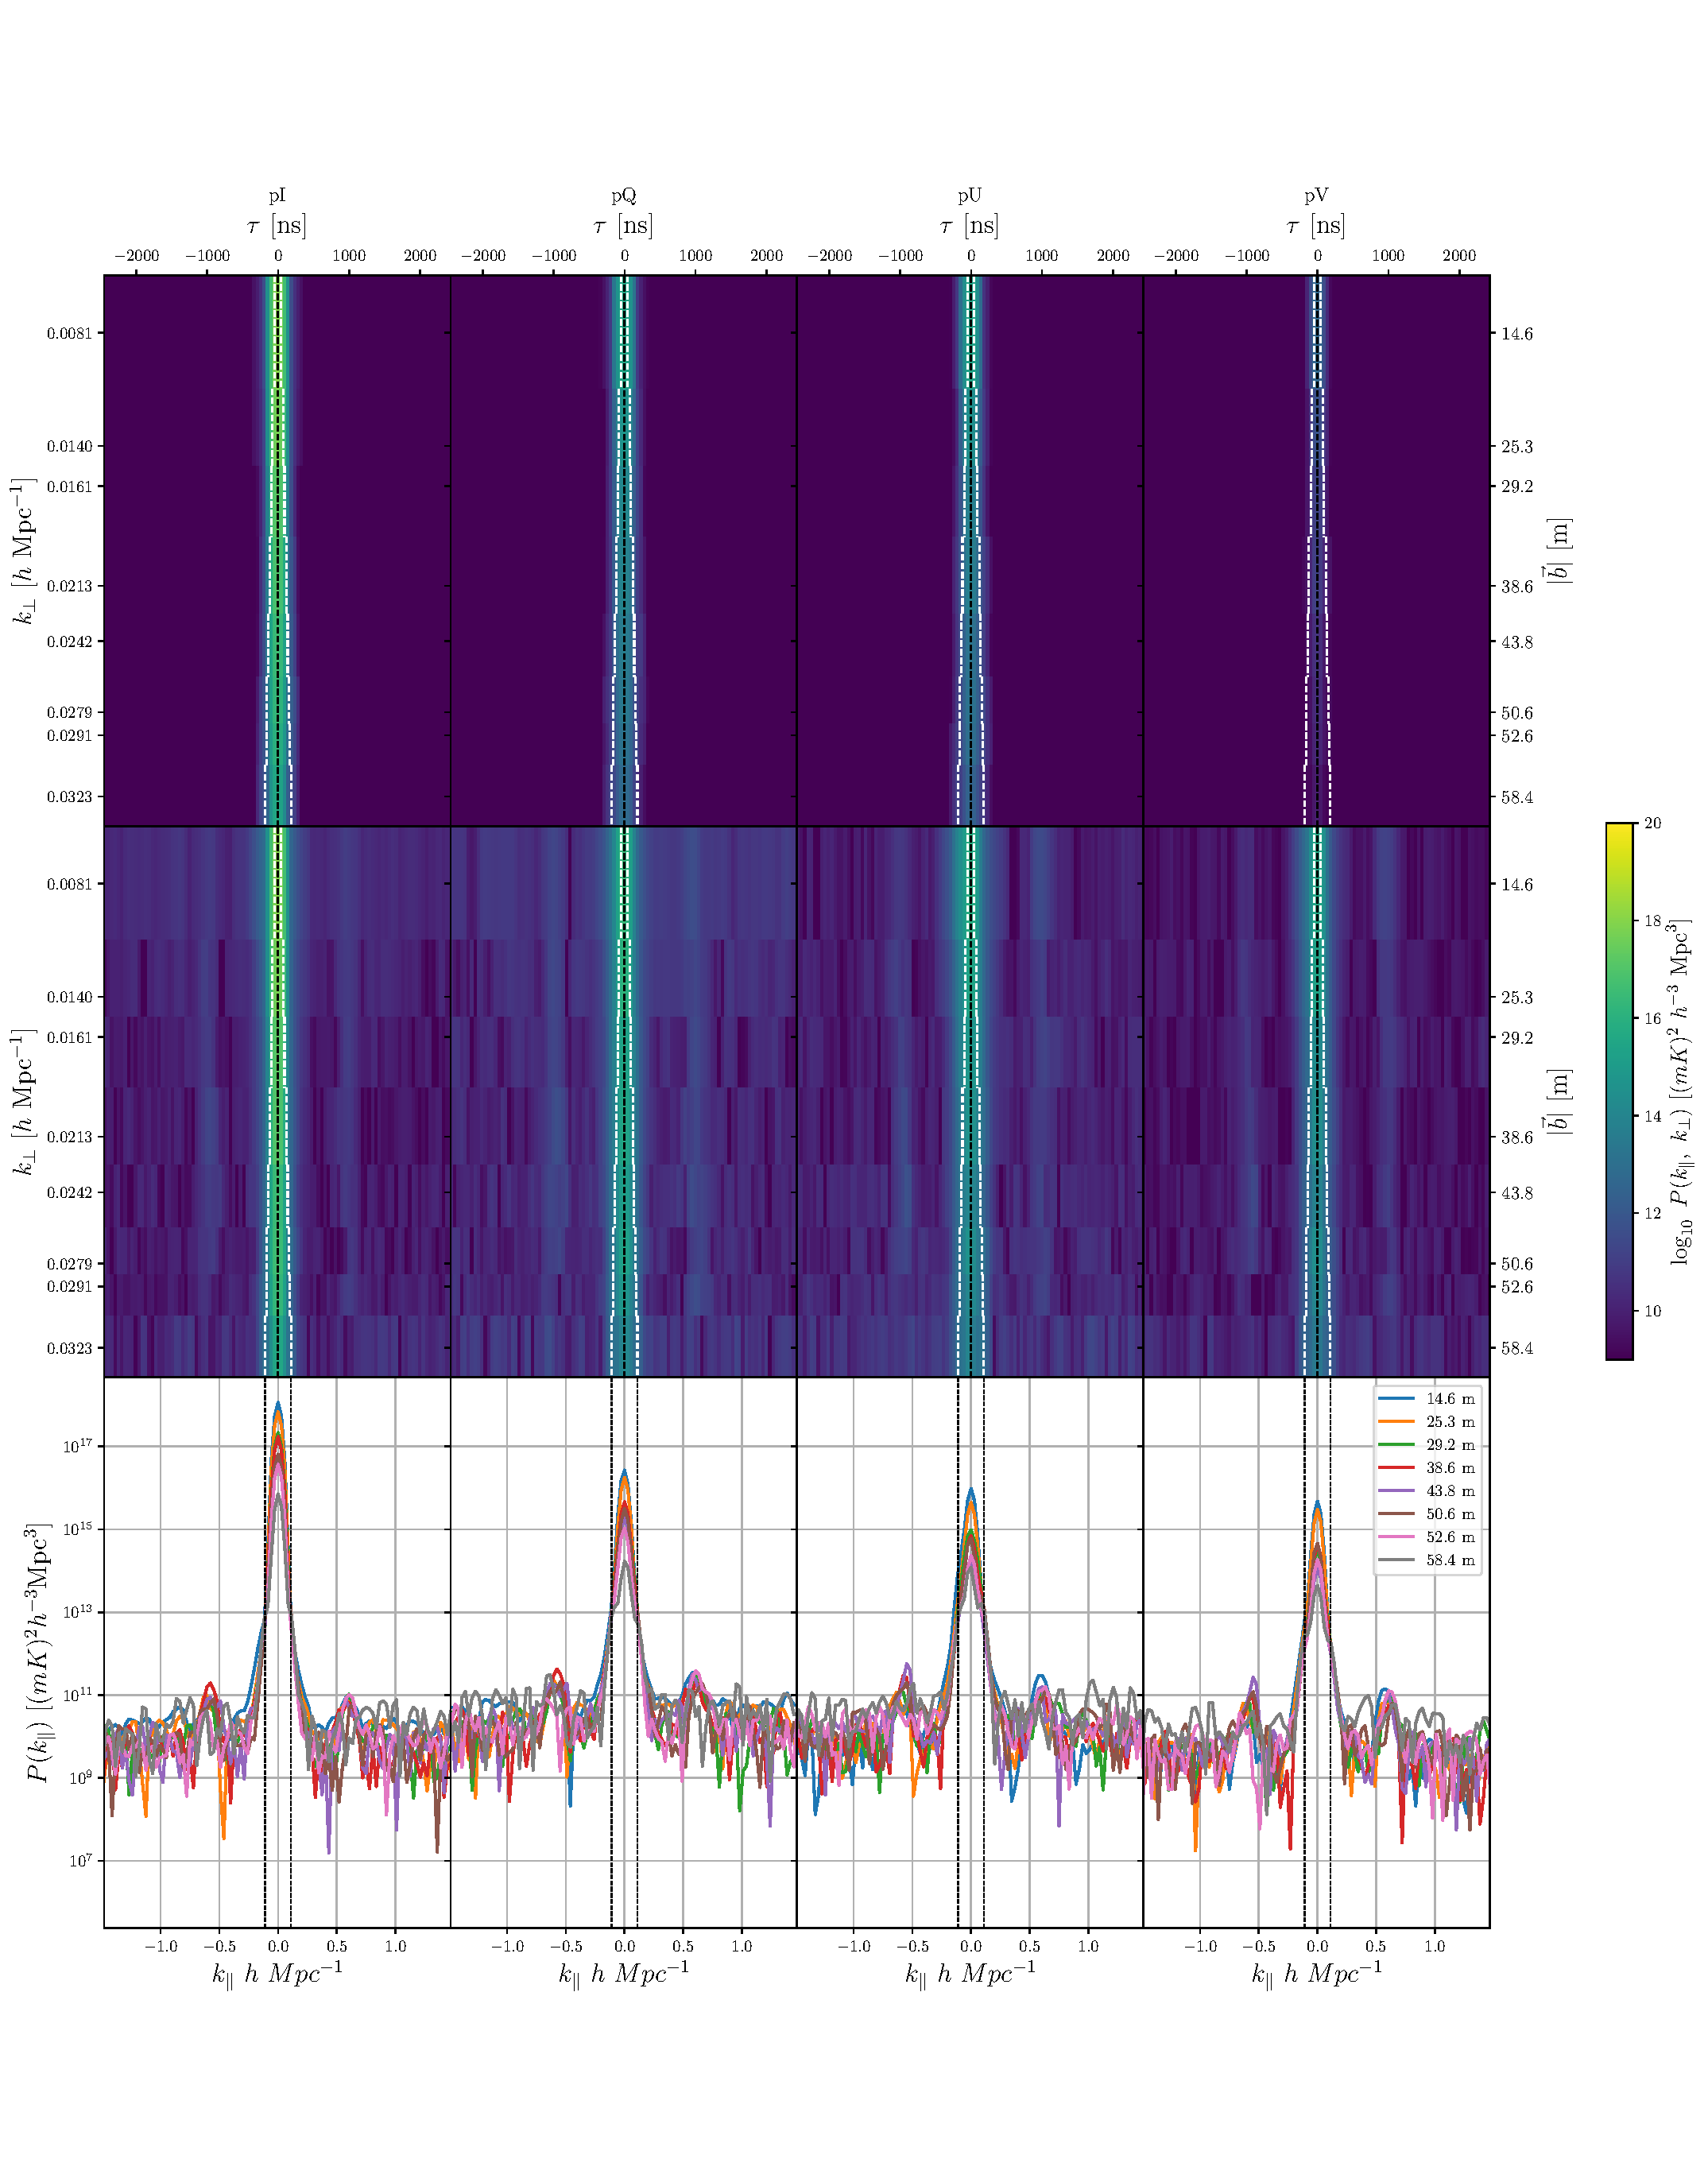
\includegraphics[scale=0.45]{highband_8day_LST_105_230.pdf}
\caption{Results from the high-band (157--167 MHz).  \textit{Top}: Simulated power spectra in Stokes I, Q, U and V, following the formalism in Section~\ref{sec:leak} -- no polarized sky model was used, so power in Stokes Q, U and V is only due to direction-dependent leakage from Stokes I.  No instrumental noise was included in the simulation. \textit{Middle}: Eight-day average power spectra from data. \textit{Bottom}: The same data as shown in the middle panel, but with each baseline length overlaid on one another to allow shared features to be more easily identified.  For the top and middle plots, white dotted lines indicate the boundary of the pitchfork and the EoR window for that baseline length. A black dotted line indicates the $k_{\parallel}=0$\,h/Mpc line.  In the bottom panel, dotted lines indicate the boundary of the wedge for the longest baseline only.
}
\label{fig:pitchforks_highband}
\end{figure*}

\begin{figure*}[h]
\centering
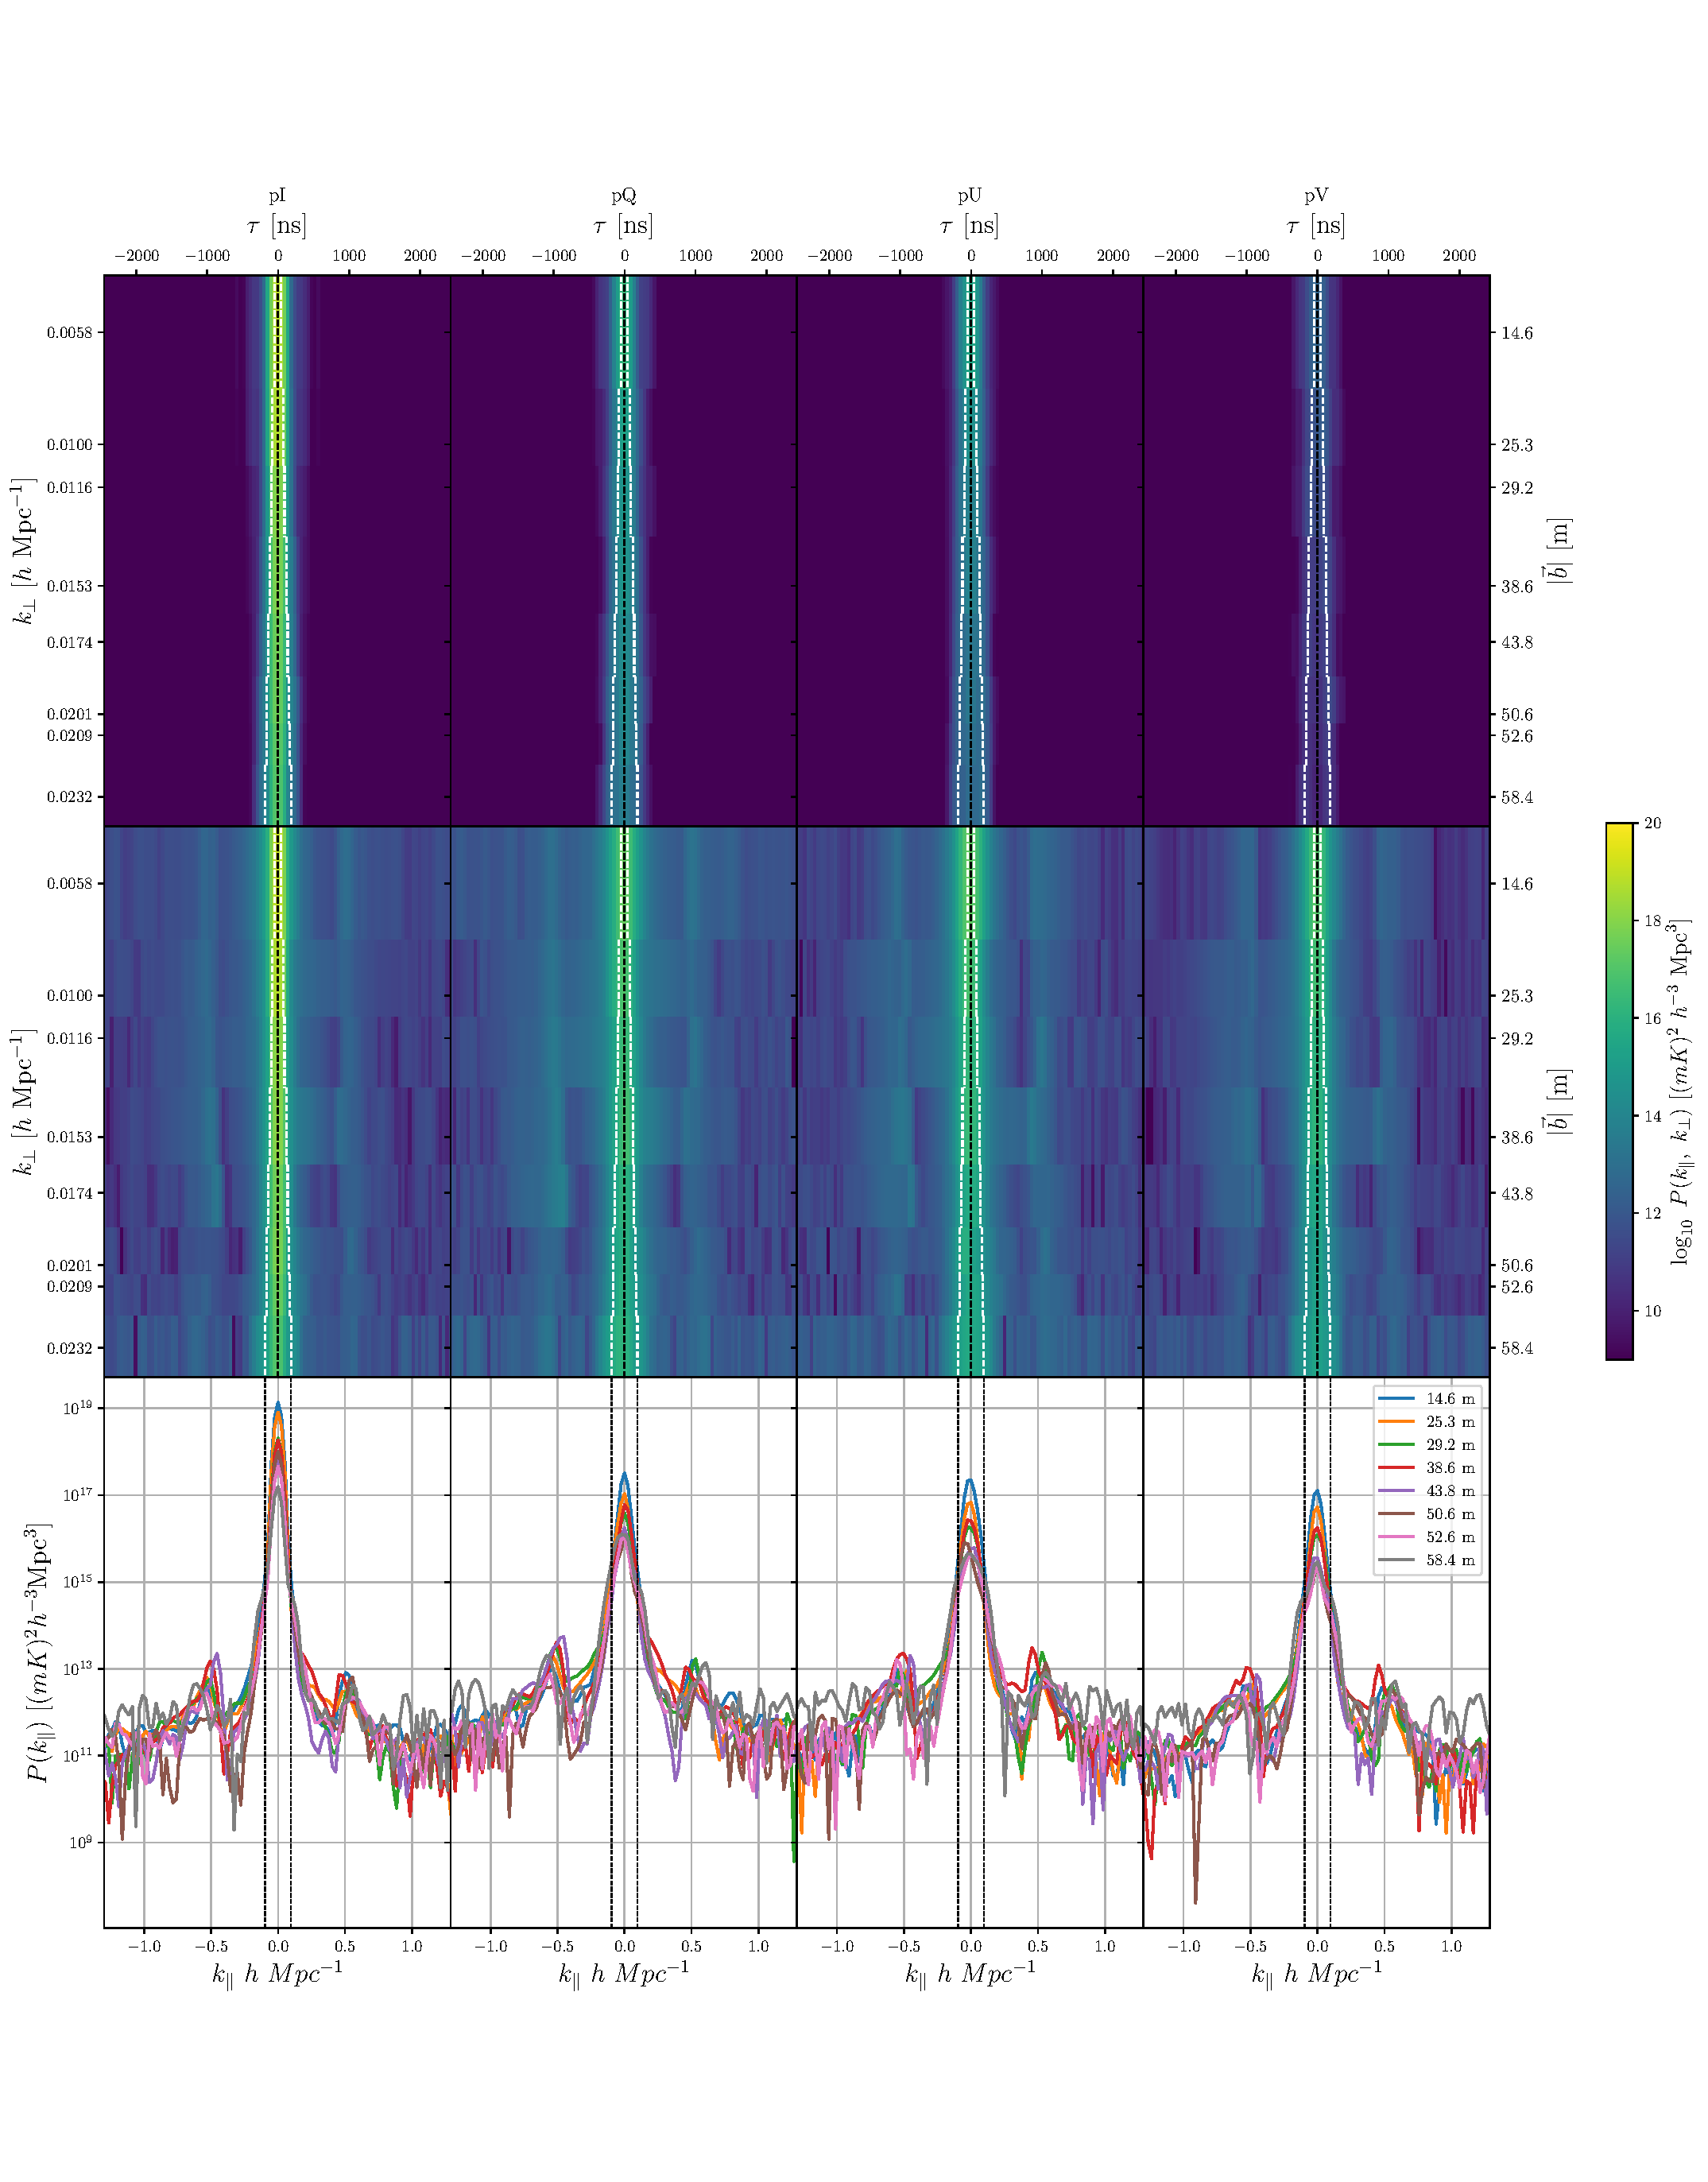
\includegraphics[scale=0.45]{lowband_8day_LST_105_230.pdf}
\caption{Results from the low-band (120--130 MHz), arranged in the same format as Figure~\ref{fig:pitchforks_highband}.}
\label{fig:pitchforks_lowband}
\end{figure*}

\clearpage

\subsection{General features of the power spectra}
\label{subsec:general_features}

\edited{
Several features of the power spectra are readily apparent.  The first is that foreground emission appears in a relatively	 narrow band near $k_\parallel = 0$.  Another is that the the shape of the power spectrum as a function of $k_\parallel$ is both sharply peaked and relatively featureless.  We note that a similar study of 2D polarized power spectra in \citet{Kohn16}, PAPER measurements showed a comparably ``filled'' region of Fourier space out to the horizon delay (i.e., to directions corresponding to zenith angle $\pm$90$^{\circ}$), with some supra-horizon leakage \citep[e.g.,][]{Pober13} into the EoR window itself. The power spectra in Figures~\ref{fig:pitchforks_highband} and \ref{fig:pitchforks_lowband} show similar behavior, though in this case the reason is the low spectral resolution ($\sim100$ ns; see Section \ref{subsec:pspec}) of the delay transform (Equation \ref{eq:DelaySpectrum}) and the small horizon delay associated with the short baselines of the array.   Thus we are not able to verify the prediction of \citet{Nithya.15b} and \citet{Neben.16} that for dishes such as HERA, the region between a delay of about 50 ns (set by the width of the antenna primary beam) and the horizon should be free of foreground emission.  Similarly, an ``excess'' of power near the horizon delay, as predicted by the same authors,
%\cite{Nithya.15b} and \cite{Neben.16}, 
is not observed, again due to the resolution in $k_\parallel$.  

Also visible in the observational data is an excess of power which is independent of the baseline length or the frequency band, and corresponds to a delay of $\sim1000 \, \mathrm{ns}$.  There are $\sim 150 \, \mathrm{m}$ coaxial cables connecting the HERA dishes to the correlator\footnote{This stage of the signal chain is only present in the commissioning array. Future HERA build-outs will transition to a different architecture using RF over fiber with long fiber runs to move this signal to even longer delays \citep{deBoer17}.} and we have good evidence that a reflection at this stage of the signal chain produces an alias of the foreground signal as observed; see \href{http://reionization.org/wp-content/uploads/2013/03/HERA39_H1C_cable_reflections_ewall-wice.pdf}{\edited{\underline{HERA Memo \#39}}} \citep{hera_memo39}.

\subsection{Comparison to Simulations}

Other features of the power spectra compare well to the simulations.  For example, the amplitude declines as a function of $k_\perp$, as expected for diffuse Galactic emission with a power law angular power spectrum.  In general, the agreement for the polarization (Q, U, V) between simulation and data is poorer.  We show a direct comparison between the power spectra of the data and the simulations for the shortest baseline length and all Stokes parameters for both bands in Figure \ref{fig:bl0_cuts_vs_sim}.

In comparing to the foreground simulations, there are two things to notice: the {\it isolation}, or the degree to which the foregrounds remain within the wedge defined by the horizon, and which can be characterized by the width of the foregrounds in $k$ (or $\tau$) space; and the {\it dynamic range}, or the ratio between the $k=0$ peak and smallest value of the power spectrum, limited measurement, either noise or artifacts from the Blackman-Harris window.}



The isolation, as measured by the simulations presented here

The lack of horizon power is corroborated by the simulations of the HERA delay response in \cite{Ewall-Wice.16} and \cite{Thyagarajan.16}, although those studies used a different windowing function for the delay transform. 

\begin{figure*}[h]
\centering
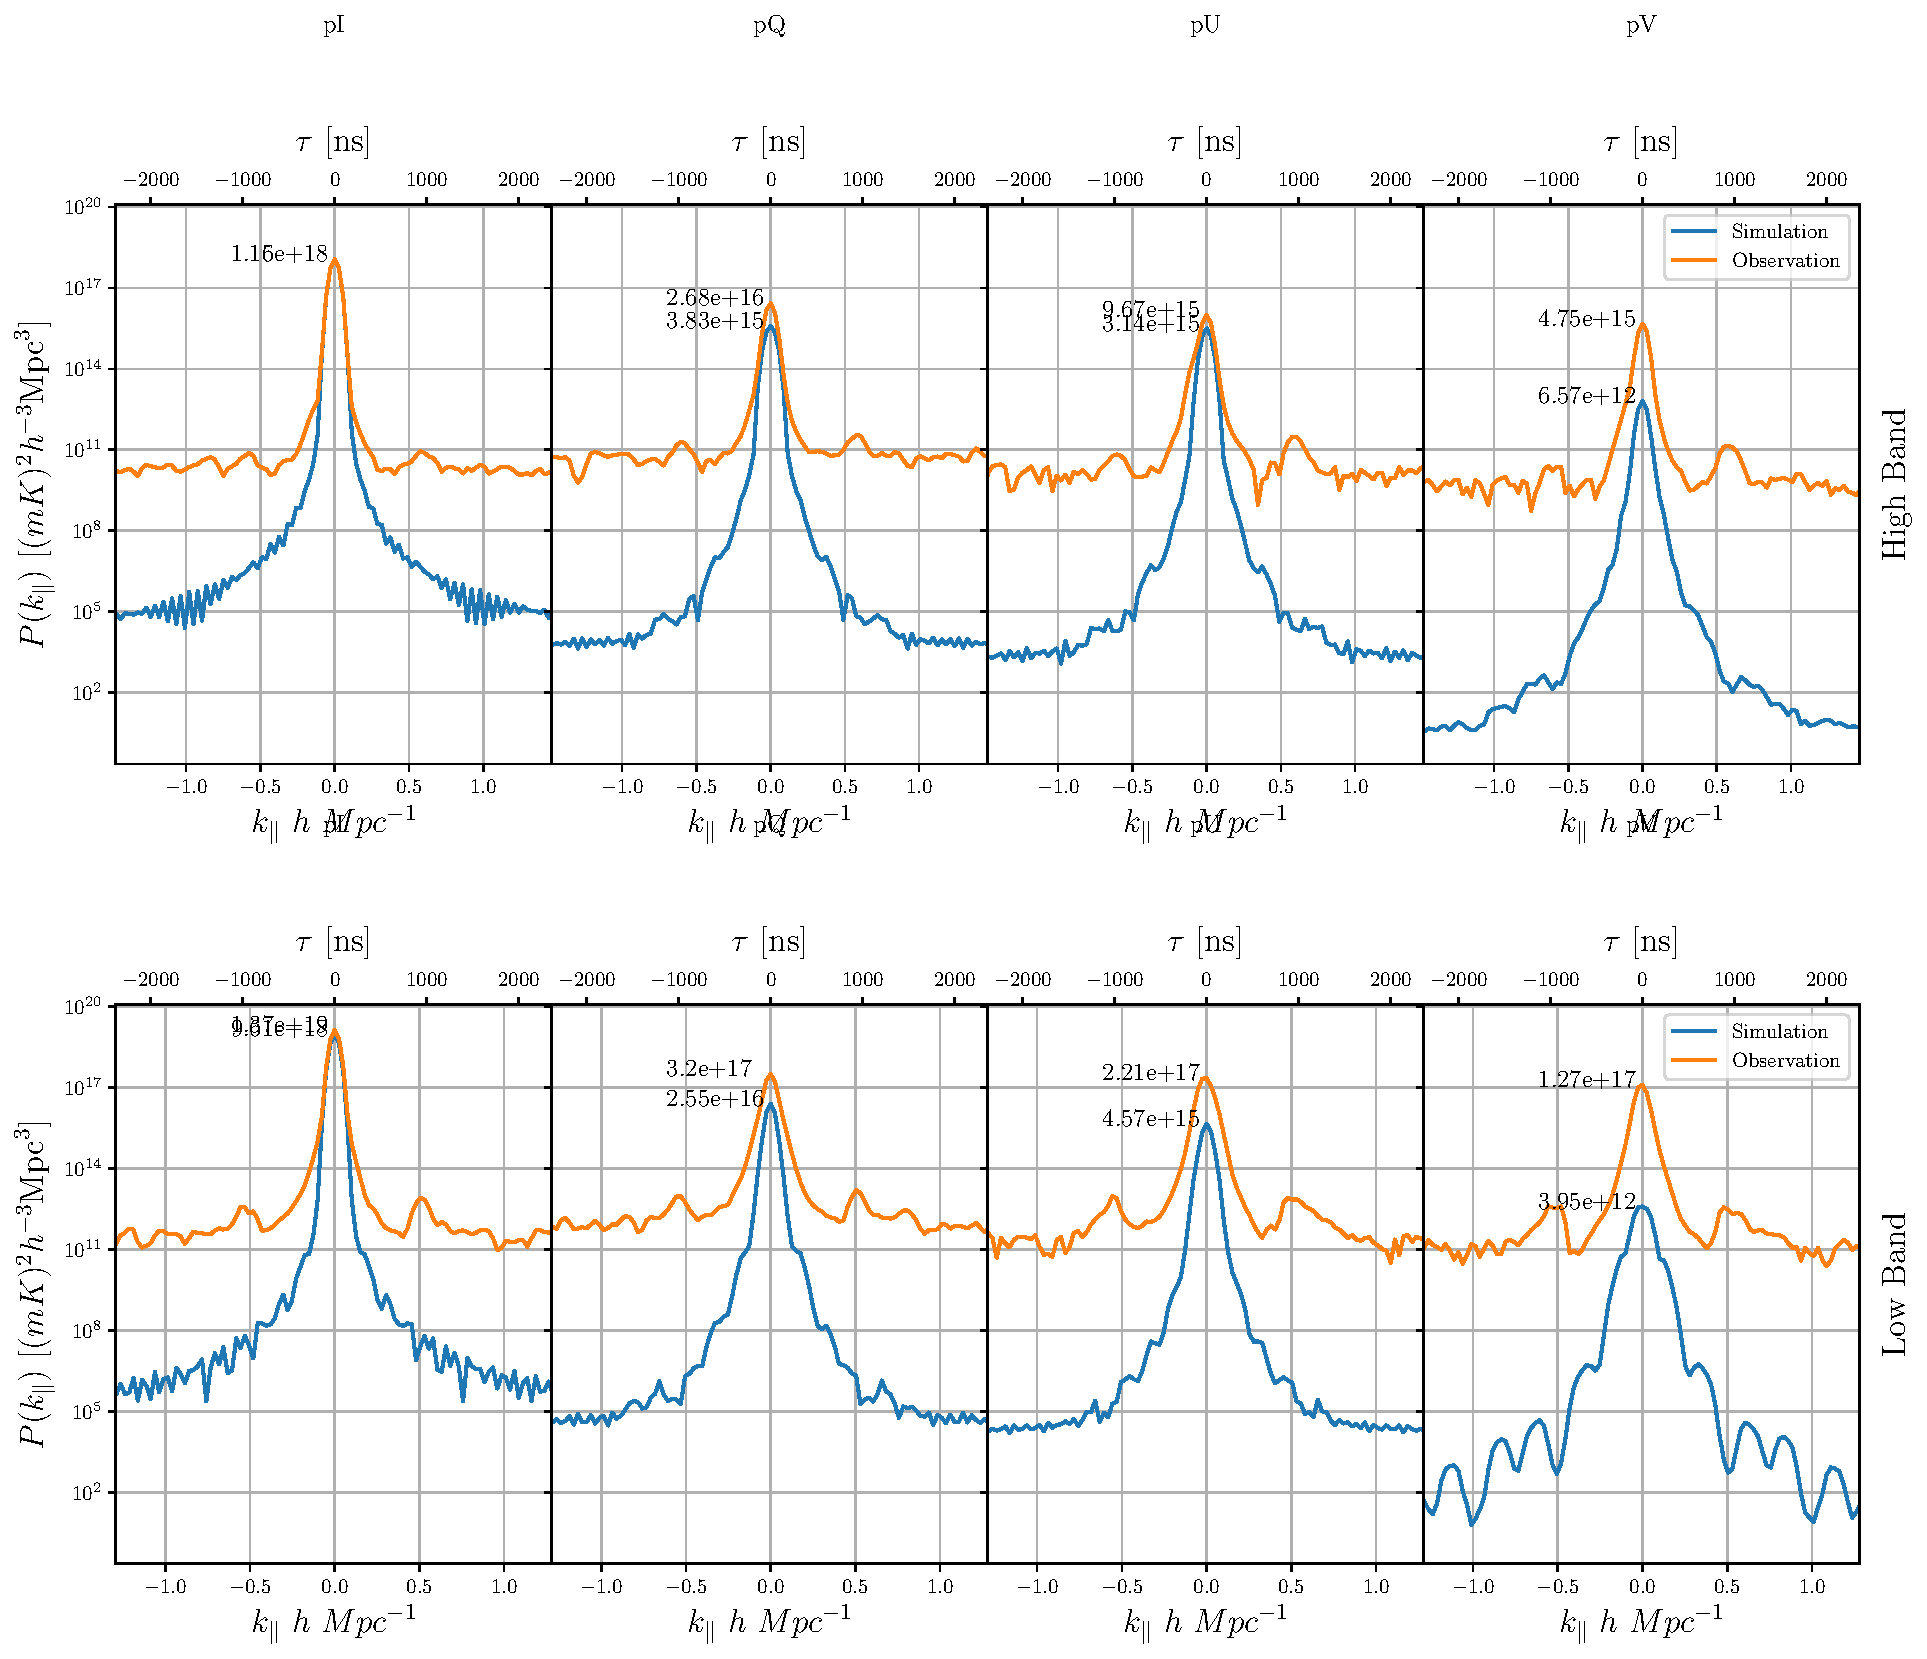
\includegraphics[width=0.9\textwidth]{real_sim_compare_noinset.pdf}
%{bl0_highband_nozoom.pdf}\\
%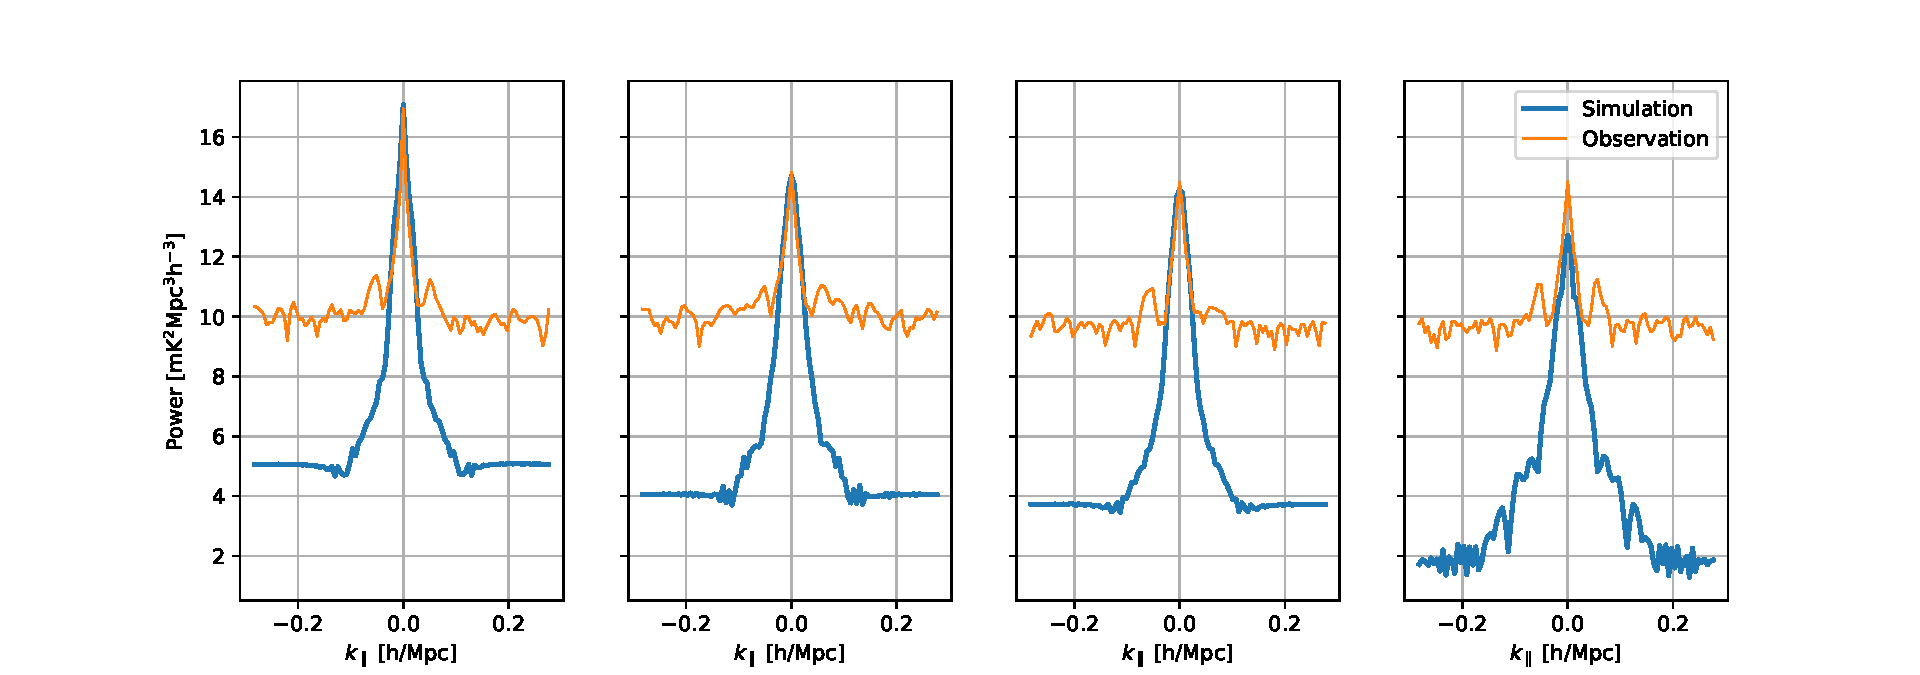
\includegraphics[width=0.9\textwidth]{bl0_lowband_nozoom.pdf}
\caption{Simulated and observed power as a function of $k_{\parallel}$ for the shortest baseline (14.6\,m). \textit{Right to left}: pseudo-Stokes I, Q, U and V; \textit{above}: the high band; \textit{below}: the low band. The simulations were noiseless and used an unpolarized sky model. They capture the foreground power levels in pseudo-Stokes I, Q and U, suggesting most power in Q and U is due to leakage from Stokes I. The power level in V is highly discrepant, however, suggesting some sort of beam-independent instrumental leakage.}
\label{fig:bl0_cuts_vs_sim}
\end{figure*}


\begin{figure*}[h]
\centering
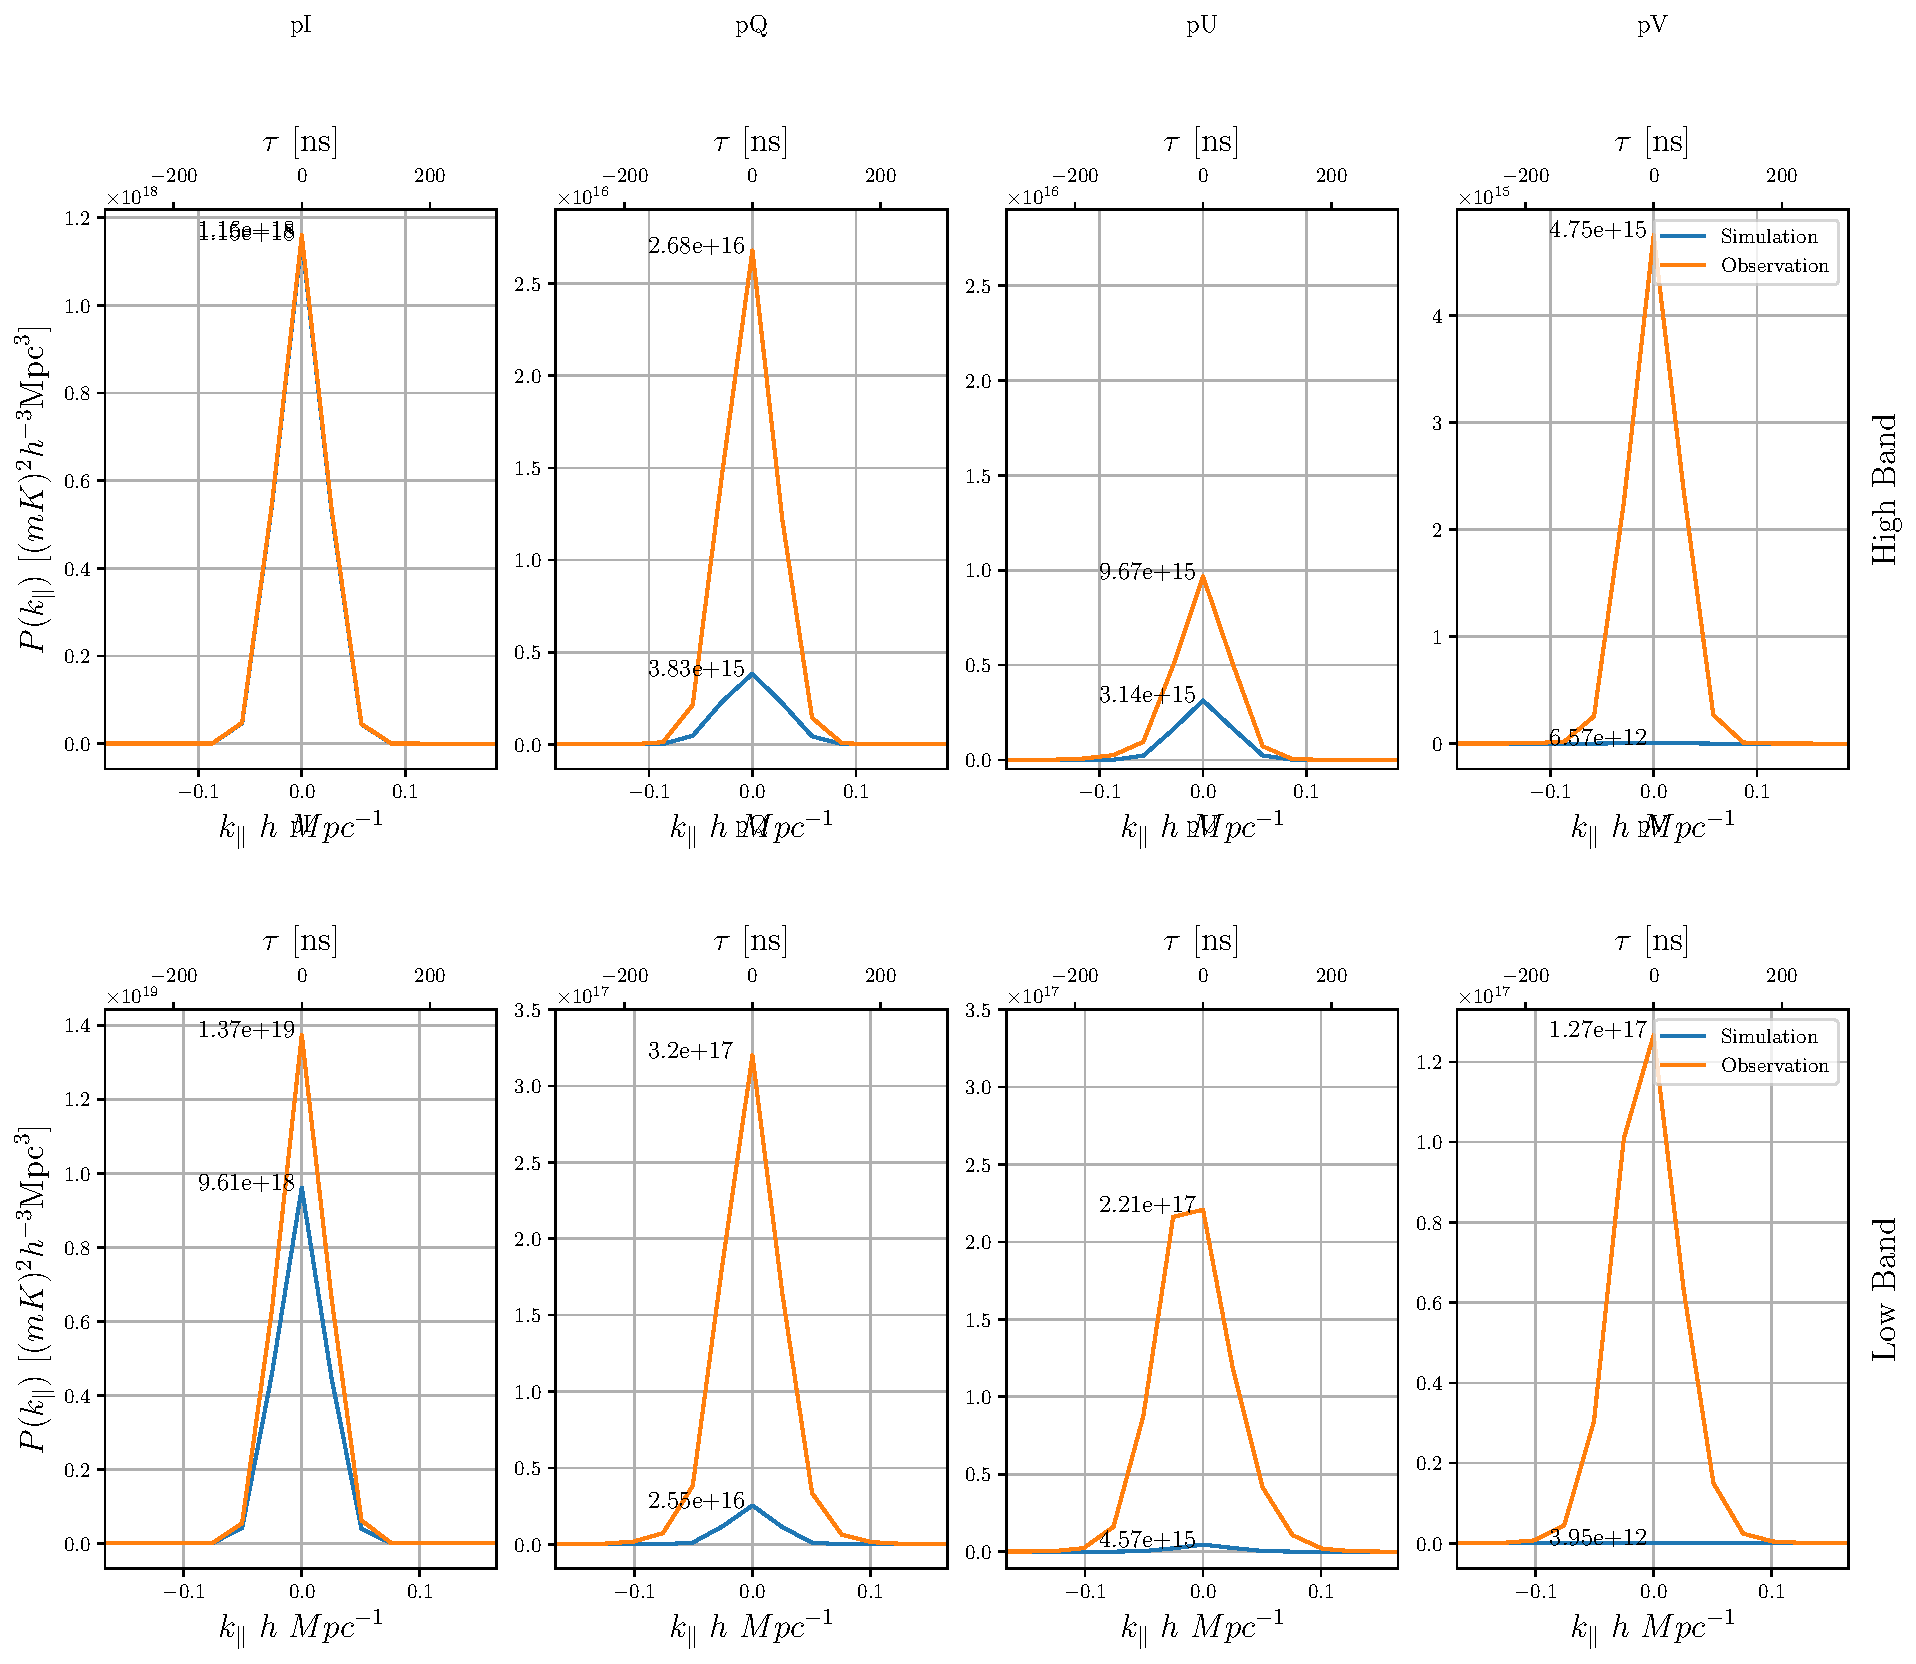
\includegraphics[width=0.9\textwidth]{ps_peak_zoom.pdf}
%{bl0_highband_nozoom.pdf}\\
%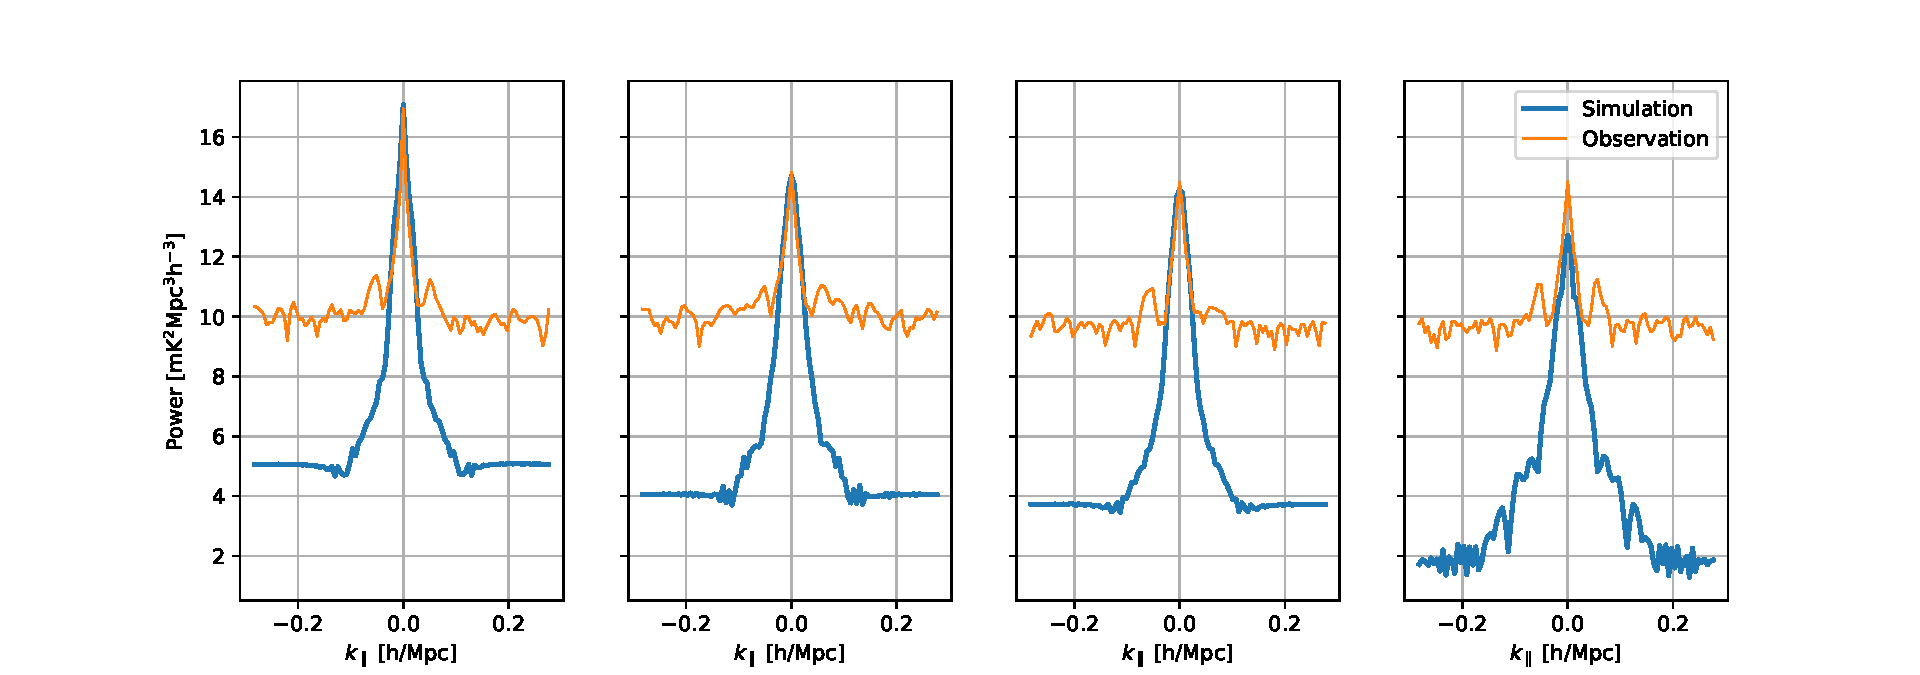
\includegraphics[width=0.9\textwidth]{bl0_lowband_nozoom.pdf}
\caption{A zoom in on Figure \ref{fig:bl0_cuts_vs_sim} showing just the $k$ values near the wedge, and with a linear scale in $P(k_\parallel)$.  
Note that the change in scales for each parameter, but also note that Q and U are set to have the same scale in each row.  
}
\label{fig:bl0_cuts_vs_sim_zoom}
\end{figure*}


\subsection{\edited{Noise Levels}}
\label{sec:Noise}

and the spectrum appears to be noise-dominated at a level approximately $10^{-8}$ of the peak.  These features match qualitatively with those obtained from the simulation.

\edited{One estimate of the system temperature of the observations was formed from the calibrated values of the auto-correlations.  These were compared against the values obtained from the simulation.  Over the RA range observed, which included the Galactic Center and much of the Galactic Plane, the average sky temperature was 2000 K \citep[][also see the public \href{http://reionization.org/wp-content/uploads/2017/04/HERA19_Tsys_3April2017.pdf}{\edited{\underline{HERA Memo \#16}}}]{deBoer17}.}

\edited{The system temperature was converted to a noise level in the power spectrum according to the formalism in \cite{Parsons.12a}, with the inclusion of a baseline-number dependence:
\begin{equation}
P_{\rm Noise}(k) \approx \frac{1}{2\Delta t \sqrt{N_{\rm LST}} N_{\rm days} N_{\rm bl}} X^2 Y B_{\rm NE} \Omega_{\rm eff} T_{\rm sys}^2.
\end{equation}
In the above equation, $\Delta t$ is integration time, $N_{\rm LST}$ is the number of LST hours used per day (12 hours), $N_{\rm bl}$ is the number of baselines (which differed per $k_{\perp}$ bin), $X$ and $Y$ are cosmological scalars defined in \cite{Parsons.12a}, $B_{\rm NE}$ is the noise equivalent bandwidth and $\Omega_{\rm eff}$ is the effective beam area, as defined in \cite{Parsons14}.  These assumptions produce a good match to the observed noise levels observed in the data; see Figure~\ref{fig:highband_cuts_per_day}.}

\subsection{Day-to-day variability}
\label{subsec:variability}

The foreground and EoR window power levels appeared to be relatively stable between days, with variation most likely due to the incomplete sky model used for gain calibration. Figure~\ref{fig:highband_cuts_per_day} shows power as a function of baseline length for $k_{\parallel}=0$ h/Mpc (solid lines) and $k_{\parallel}=0.2$ h/Mpc (dot-dashed lines). Deviations from the mean at $k_{\parallel}=0$ h/Mpc may be a limitation imposed by our simplistic sky model. Since the noise levels in the EoR window region remained noise-like throughout our observations, the uncertainty in the absolute gain scale did not have a large impact on our largely-diagnostic investigation.

\begin{figure}
\centering
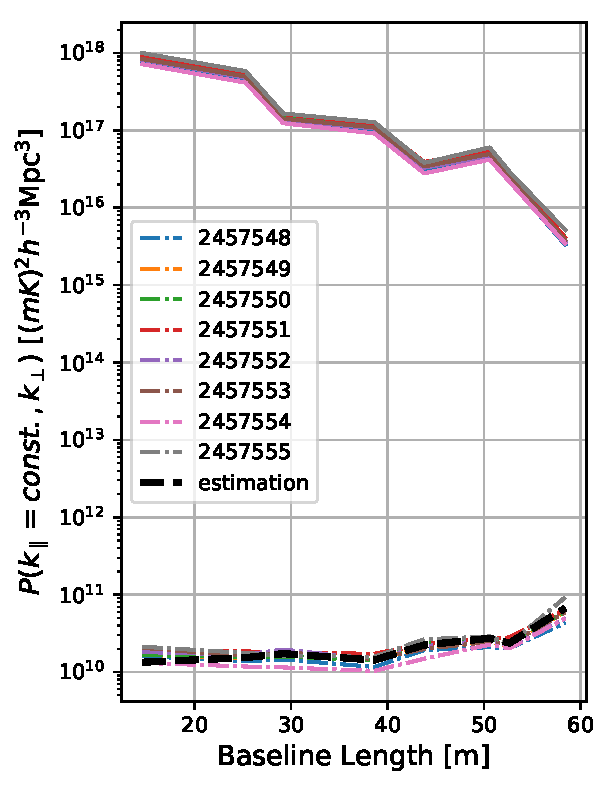
\includegraphics[width=0.9\columnwidth]{noise_estimation.pdf}
%{highband_by_day.pdf}
\caption{High band power as a function of baseline length for the center of the pitchfork ($k_{\parallel}=0$ h/Mpc; solid lines) and in the EoR window ($k_{\parallel}=0.2$ h/Mpc; dot-dashed lines) for \edited{pseudo-Stokes I on} each JD of observation. The black dashed line represents the approximate noise power assuming a receiver temperature of 300\,K. A very similar relationship is shown in the low band, but with a higher noise floor, which is consistent with system temperature as a function of frequency. The noise level climbs with baseline length as the compact nature of the array gives more short baselines to average-over in a given $(k_{\parallel},k_{\perp})$ bin than longer ones.}
\label{fig:highband_cuts_per_day}
\end{figure}

\subsection{Polarimetric results}
\label{subsec:polarimetric_results}

Figures~\ref{fig:pitchforks_highband} and~\ref{fig:pitchforks_lowband} qualitatively illustrate that the simulations described in Section~\ref{subsec:DD-Leak} reproduced the main features of the observed power spectra. The simulations were run only with a Stokes I sky component and no simulated calibration errors, so the only signal in the polarized power spectra was from wide-field beam leakage (Figure~\ref{fig:mueller}). An example comparison between simulation and observation in the image plane is shown in Figure~\ref{fig:GCimage}.

In Figure~\ref{fig:bl0_cuts_vs_sim} we show the power levels observed on the shortest baseline (14.7\,m) compared to our simulations for each band. The simulations used an unpolarized diffuse sky model \citep[the most recent version of the GSM;][]{GSM.17}, which should be accurate at the scales probed by a 14.7\,m baseline. 
%Inset panels zoom-in on the region around $k_{\parallel}=0$\,h/Mpc, where most of the foreground power was concentrated.
We saw that the simulations reproduced $\sim75\%$ of the foreground power observed in pseudo-Stokes I in the high band, and over-predicted foreground power by $\sim35\%$ in the low band. This could have been due to unrealistic frequency scaling of the diffuse foregrounds in the GSM. 

For pseudo-Stokes Q and U, the simulations accounted for $\sim 60-75\%$ of power seen within the pitchfork region, suggesting that most of the power seen in these power spectra, at least for the shortest baselines, can be mostly attributed to direction-dependent leakage effects. 
%\edited{Residual gain and phase errors are able to leak a fraction of pseudo-Stokes I into Q and U in a direction-independent fashion. There is excess power close to the location of the Galactic Center, and increased power over the sky, in the observed pseudo-Stokes Q and U skies compared to the simulated ones in Figure~\ref{fig:GCimage}. Recall that  the simulated pseudo-Stokes Q and U images contain only direction-dependent leakage from Stokes I. As the Galactic Center is the highest-amplitude source of power, we expect residual gain errors to be most obvious in the same position as it is in the pseudo-Stokes I image. 
%Such an excess is indeed present in the observed pseudo-Stokes Q and U images, but absent in the simulated ones -- pointing to direction-independent gain errors being present.}

\edited{Some fraction of the observed power ($\leqslant 25\%$; the excess in polarized power above predicted leakage levels) may have been due to linearly polarized foregrounds. Referring to Figure~\ref{fig:bl0_cuts_vs_sim}, the measured ratio of the pseudo-Stokes Q and U power spectra to pseudo-Stokes I was roughly 2.5 dex. Removing the expected $\sim75\%$ of power attributed to direction-dependent leakage, and assuming the remainder to be intrinsically polarized power rather than direction-independent gain errors, corresponded to an intrinsic polarized fraction of $\sim 0.03$. This would represent polarized fluctuations measured by the shortest baseline to be on the order of $\sim 5$K, consistent with measurements of large-scale polarized structures by \cite{Jelic.15} and \cite{Lenc.16}. To disentangle the contribution of gain errors and intrinsic polarization to the observed power requires more substantial simulation and statistical subtraction efforts \citep[e.g.][]{Lenc.18}, which is outside the scope of this paper, and we defer to future work.}

%Leave out
% Compare to Asad?
%\cite{Lenc.16} observed linearly polarized emission from diffuse structure with $\sim 1.6 - 4.5\%$ fractional polarization at 150\,MHz, corresponding to power levels of $\sim10^5$ mK$^2$Mpc$^3$h$^{-3}$. This power level is similar to expected EoR power levels \citep[e.g.][]{Lidz.07, Moore13, Nunhokee.17}; a detection of a power spectrum of polarized galactic synchrotron will require much deeper integrations.
%


The observed pseudo-Stokes V power spectrum was more poorly modelled by our simulation. In both bands we observed $\sim$20 dB more power in pseudo-Stokes V at $k_{\parallel}=0$\,h/Mpc than predicted by our simulations. The peak power observed in pseudo-Stokes V was roughly 0.1\% of the peak power observed in pseudo-Stokes I. Likewise in the sky images shown in Figure~\ref{fig:GCimage}, there is little pseudo-Stokes V power in the simulated images, compared to observation. This suggests that most or all of the power in pseudo-Stokes V is due to direction independent leakage. While the leakage appears localized in Figure~\ref{fig:GCimage}, we see in Figure~\ref{fig:bl0_cuts_vs_sim} that it is statistically similar to pseudo-Stokes Q and U in power.
Since $D$-terms cause direction-independent leakage from pseudo-Stokes I to pseudo-Stokes V, the excess power we observed could be interpreted as an approximate $D$-term level of $\sim$1\% \citep{TMS}. This is similar to $D$-term levels from other low frequency instruments such as MWA-32, which was found to have $\sim$2\% $D$-terms (G. Bernardi, private communication).
To understand which effect, if either, is dominant, a precise $D$-term calibration of HERA is required. This effort is underway with data taken with bright polarized point sources in transit, and will be presented in future work. Another potential cause of the discrepancy could have been that our simulations under-predicted Stokes V power, due to lack of accounting for some variety of instrumental circular polarization.

In Section~\ref{subsec:general_features} we noted the presence of excess power at $k_{\parallel}=\pm 0.04$\,h/Mpc ($\pm$100\,ns) that was independent of baseline length, suggesting that it was due to a reflection along 15\,m cables. Figure~\ref{fig:bl0_cuts_vs_sim} shows that power at this delay is not consistent between polarizations. Stokes U and V power only exhibited excess signal at -100\,ns in the high band, and in the low band, it was only Stokes U that did not exhibit that excess at +100\,ns. This may be a clue about the polarization state of cable reflections, perhaps as a function of frequency, but we defer this to future work -- noting it as a point of interest here.

\edited{\section{Conclusions}}
\label{conc}

In this work we have presented polarized power spectra from the HERA-19 commissioning array. With modest calibration, HERA is able isolate total intensity and polarized foregrounds to within the ``pitchfork'' region of \textit{k}-space, as predicted by \cite{Nithya.15b}, lending confidence to its future performance as an instrument capable of both detecting and characterizing the EoR power spectrum. Of course, the array used in this study had just 19 antennae, 15 of which were used for analysis -- future build-outs of HERA with up to 350 antennae will require strong quality-assurance efforts. %Larger HERA build-outs will also provide more $k_{\perp}$-modes 

Simulations of the polarized response of the instrument, mapped into the same Fourier space as the data, suggest that most or all of the polarized power observed in pseudo-Stokes Q and U power spectra is due to direction-dependent beam leakage from pseudo-Stokes I. Residual gain and phase errors could account for the rest of the power, but some fraction of the total ($\leqslant 25\%$) may be due to linearly polarized foregrounds. Excess power in pseudo-Stokes V may be due to $D$-terms at the 1\% level, but a full image-based calibration with a polarized point source is required to confirm this. The general accuracy of our simulations suggests current modeling of the complex HERA beam is accurate.

\acknowledgements

Much of this study was undertaken during the inaugural CAMPARE-HERA Astronomy Minority Partnership (CHAMP).
This material is based upon work supported by the National Science Foundation under Grant Nos. 1440343 and 1636646, the Gordon and Betty Moore Foundation, and institutional support from the HERA collaboration partners.
SAK is supported by a University of Pennsylvania SAS Dissertation Completion Fellowship.
JEA acknowledges support from NSF CAREER award \# 1455151.
C.D.N. is supported by the SKA SA scholarship program.
AL acknowledges support for this work by NASA through Hubble Fellowship grant \# HST-HF2-51363.001-A awarded by the Space Telescope Science Institute, which is operated by the Association of Universities for Research in Astronomy, Inc., for NASA, under contract NAS5-26555.
G.B. acknowledges support from the Royal Society and the Newton Fund under grant NA150184. This work is based on the research supported in part by the National Research Foundation of South Africa (grant No. 103424).
JSD acknowledges the support of the NSF AAPF award \# 1701536 and the Berkeley Center for Cosmological Physics.

We thank the anonymous referee for many helpful suggestions.

\software{This research made use of Astropy, a community-developed core Python package for Astronomy \citep{astropy13}; CASA \citep{casa}; pyuvdata \citep{pyuvdata}; pygsm \citep{pygsm} }

\clearpage

\bibliography{mybib}
\bibliographystyle{apj}

\end{document}